\RCS$Revision: $
\RCS$HeadURL: $
\RCS$Id: $

%_______________________________________________________________________________
%_______________________________________________________________________________
%_______________________________________________________________________________

%\newcommand{\kfactor}{\ensuremath{k\text{-factor}}\xspace}
\newcommand{\kfactors}{\ensuremath{k\text{-factors}}\xspace}
\newcommand{\njet}{\ensuremath{n_{\text{jet}}}\xspace}
\newcommand{\njetlow}{\ensuremath{2 \leq \njet \leq 3}\xspace}
\newcommand{\njethigh}{\ensuremath{\njet \geq 4}\xspace}
\newcommand{\nb}{\ensuremath{n_{\text{b}}}\xspace}
\newcommand{\alphat}{\ensuremath{\alpha_{\text{T}}}\xspace}
\newcommand{\alphatcut}{\ensuremath{\alpha_{\text{T}}^{\text{cut}}}\xspace}
\newcommand{\htalphat}{\texttt{HT\_AlphaT}\xspace}
\newcommand{\photon}{\texttt{Photon}\xspace}
\newcommand{\muht}{\texttt{Mu\_HT}\xspace}
\newcommand{\httrigger}{\texttt{HT}\xspace}
\newcommand{\mt}{\ensuremath{M_{\textrm T}}\xspace}
\newcommand{\gj}{\ensuremath{\gamma} + jets\xspace}
\newcommand{\mj}{\ensuremath{\mu} + jets\xspace}
\newcommand{\mmj}{\ensuremath{\mu\mu} + jets\xspace}
\newcommand{\npre}{\ensuremath{N_{\textrm{pred}}}\xspace}
\newcommand{\nobs}{\ensuremath{N_{\textrm{obs}}}\xspace}
\newcommand{\njets}{\ensuremath{N_{\textrm{jet}}}\xspace}
\newcommand{\sq}{\ensuremath{\tilde{\rm q}}\xspace}
\newcommand{\st}{\ensuremath{\tilde{\rm t}}\xspace}
\newcommand{\gl}{\ensuremath{\tilde{\rm g}}\xspace}
\newcommand{\dht}{\ensuremath{\Delta\scalht}\xspace}
\newcommand{\ewk}{\ensuremath{\mathrm{EWK}}\xspace}
\newcommand{\qcd}{\ensuremath{\mathrm{QCD}}\xspace}
\newcommand{\fZinv}[1]{\ensuremath{f_{\rm Zinv}^{#1}}\xspace}
\newcommand{\zInv}[1]{\ensuremath{Z_{\rm inv}^{#1}}\xspace}
\newcommand{\meanHt}[1]{\ensuremath{\langle \HT \rangle^{#1}}\xspace}
\newcommand{\lk}[2]{\ensuremath{L^{\rm #1}_{\rm #2}}\xspace}
\newcommand{\sep}{\ensuremath{68^{\mathrm{th}}}\xspace}
\newcommand{\partonht}{\ensuremath{\scalht^{\rm parton}}\xspace}
\newcommand{\meff}{\ensuremath{M_{\rm eff}}\xspace}
\newcommand{\mhttt}{\ensuremath{\hslash_{\rm T}^{TT}}\xspace}


%\newcommand\rs{\raisebox{1.0ex}[-1.0ex]}
\newcommand{\ra}{\ensuremath{\rightarrow}}
\newcommand{\znunu}{\ensuremath{{\text Z} \ra \nu\bar{\nu}}\xspace}
\newcommand{\zll}{\ensuremath{{\text Z} \ra \ell\ell}\xspace}
\newcommand{\zmumu}{\ensuremath{{\text Z} \ra \mu\mu}\xspace}
\newcommand{\zee}{\ensuremath{{\text Z} \ra ee}\xspace}
\newcommand{\wmunu}{\ensuremath{{\text W} \ra \mu\nu}}
\newcommand{\wtaunu}{\ensuremath{{\text W} \ra \tau\nu}}
\newcommand{\dphi}{\ensuremath{\Delta \phi}}
\newcommand{\dphijj}{\ensuremath{\Delta \phi_{ j1,j2}}}
\newcommand{\Pt}{\ensuremath{{p_{\text T}}}\xspace}
\newcommand{\pts}{\ensuremath{p_{\text T}{\text s}}\xspace}
\newcommand{\Et}{\ensuremath{{E_{\text T}}}\xspace}
\newcommand{\ptjf}{\ensuremath{p_{\rm T}^{ {\rm j}_1} }}
\newcommand{\ptjs}{\ensuremath{p_{\rm T}^{ {\rm j}_2} }}
\newcommand{\ptjt}{\ensuremath{p_{\rm T}^{ {\rm j}_3} }}
\newcommand{\etajf}{\ensuremath{\eta^{ {\rm j}_1} }}
\newcommand{\etajs}{\ensuremath{\eta^{ {\rm j}_2} }}
\newcommand{\etajt}{\ensuremath{\eta^{ {\rm j}_3} }}
\newcommand{\ttj}{\ensuremath{\rm{t}\bar{\rm{t}} + jets}\xspace}
\newcommand{\wj}{\ensuremath{\rm W + \textrm{jets}}\xspace}
\newcommand{\wej}{\ensuremath{{\rm W}(\rightarrow{\rm e}\nu) + \textrm{jets}}\xspace}
\newcommand{\wmj}{\ensuremath{{\rm W}(\rightarrow\mu\nu) + \textrm{jets}}\xspace}
\newcommand{\zj}{\ensuremath{{\rm Z} + \textrm{jets}}\xspace}
\newcommand{\zmmj}{\ensuremath{{\rm Z}(\rightarrow\mu\mu) + \textrm{jets}}\xspace}
\newcommand{\zeej}{\ensuremath{{\rm Z}(\rightarrow{\rm ee}) + \textrm{jets}}\xspace}

\newcommand{\al}{\ensuremath{\alpha}}
\newcommand{\alt}{\ensuremath{\alpha_{\text{T}}}\xspace}
\newcommand{\etaabs}{\ensuremath{|\eta|}}
%\newcommand{\gev}{\ensuremath{\mathrm{\,Ge\kern -0.1em V}}}
\newcommand{\pb}{\ensuremath{pb^{-1}}}
\newcommand{\mjj}{\ensuremath{M_{\text{inv}}^{j1,j2}}}
%\newcommand{\ttbar}{\ensuremath{t\bar{t}}}
\newcommand{\chiznew}{\ensuremath{\chi^{0}}\xspace}
\newcommand{\chipnew}{\ensuremath{\chi^{+}}\xspace}
\newcommand{\sQuanew}{\ensuremath{\tilde{\rm q}}\xspace}
\newcommand{\sGlunew}{\ensuremath{\tilde{\rm g}}\xspace}
\newcommand{\ttNew}{\ensuremath{\rm{t}\bar{\rm{t}}}\xspace}
\newcommand{\tev}{\TeV}
%<TW date="30/10/2010">
%\newcommand{\Et}{E_{T}}
\newcommand{\combIso}{Iso_{\textrm{comb.}}}
\renewcommand{\arraystretch}{1.2}
\newcommand{\bigNum}[2]{#1 \, \times \, 10 \, ^{#2}}
%</TW>

\newcommand{\raT}{\ensuremath{R_{\alt}}}
\newcommand{\RaT}{\ensuremath{R_{\alt}}\xspace}

\newcommand{\Ttwocc}{\ensuremath{\text{pp}\,\ra\,\sTop\sTop^{*}\,\ra\,\text{c}\chiz\,\bar{\text{c}}\chiz}}
\newcommand{\Ttwodegen}{\ensuremath{\text{pp}\,\ra\,\sTop\sTop^{*}\,\ra\,\text{b}ff'\chiz \,\text{b}ff'\chiz}}
\newcommand{\Ttwobw}{\ensuremath{\text{pp}\,\ra\,\sTop\sTop^{*}\,\ra\,\text{b}W\chiz \,\bar{\text{b}}W\chiz}}
\newcommand{\Ttwott}{\ensuremath{\text{pp}\,\ra\,\sTop\sTop^{*}\,\ra\,\text{t}\chiz\,\bar{\text{t}}\chiz}}
\newcommand{\Ttwobb}{\ensuremath{\text{pp}\,\ra\,\sBot\sBot^{*}\,\ra\,\text{b}\chiz\,\bar{\text{b}}\chiz}}
\newcommand{\Ttwoqq}{\ensuremath{\text{pp}\,\ra\,\sQua\sQua^{*}\,\ra\,\text{q}\chiz\,\bar{\text{q}}\chiz}}
\newcommand{\Tonebbbb}{\ensuremath{\text{pp}\,\ra\,\sGlunew\sGlunew^{*}\,\ra\,\bar{\text{b}}\text{b}\chiz\,\bar{\text{b}}\text{b}\chiz}}
\newcommand{\Toneqqqq}{\ensuremath{\text{pp}\,\ra\,\sGlunew\sGlunew^{*}\,\ra\,\bar{\text{q}}\text{q}\chiz\,\bar{\text{q}}\text{q}\chiz}}
\newcommand{\Tonetttt}{\ensuremath{\text{pp}\,\ra\,\sGlunew\sGlunew^{*}\,\ra\,\bar{\text{t}}\text{t}\chiz\,\bar{\text{t}}\text{t}\chiz}}

\newcommand\T{\rule{0pt}{2.6ex}}
\newcommand\B{\rule[-1.2ex]{0pt}{0pt}}

\def\eslash{{\hbox{$E$\kern-0.6em\lower-.05ex\hbox{/}\kern0.10em}}}
\def\vecmet{\mbox{$\vec{\eslash}_T$}} %missing ET vector
\def\vecet{\mbox{$\vec{E}_\text{T}$}} % ET vector
\def\MET{\mbox{$\eslash_\text{T}$}\xspace}
%\def\met{\mbox{$\eslash_\text{T}$}\xspace}
\def\met{\mbox{$E_\text{T}^{\rm miss}$}\xspace}
\def\pfmet{\mbox{$\eslash_\text{T}^{\rm PF}$}\xspace}
\def\mex{\mbox{$\eslash_\text{x}$}} %missing Ex
\def\mey{\mbox{$\eslash_\text{y}$}} %missing Ey
\def\mepar{\mbox{$\eslash_\parallel$}}
\def\meperp{\mbox{$\eslash_\perp$}}
\def\Zmm{Z \rightarrow \mu\mu}
\def\metvec{\mbox{$\vec{\met}$}\xspace}
\def\metvecrec{\mbox{$\vec{\met}^{\rm rec}$}\xspace}
\def\metvecgen{\mbox{$\vec{\met}^{\rm gen}$}\xspace}
\def\metgen{\mbox{$\met^{\rm gen}$}\xspace}
\def\metparl{\mbox{$\mepar^{\rm rec}$}\xspace}
\def\metperp{\mbox{$\meperp^{\rm rec}$}\xspace}
\def\deltamet{\mbox{$\Delta\met$}\xspace}
\def\pthat{\mbox{$\hat{p}_T$}\xspace}
\def\hslash{{\hbox{$H$\kern-0.8em\lower-.05ex\hbox{/}\kern0.10em}}}
\def\MHT{\mbox{$\hslash_\text{T}$}\xspace}
%\def\mht{\mbox{$\hslash_\text{T}$}\xspace}
\def\mht{\mbox{$H_{\rm T}^{\rm miss}$}\xspace}
\def\mhtvec{\mbox{$\vec{H}_{\rm T}^{\rm miss}$}\xspace}
%\def\mhtmet{\mbox{$\hslash_\text{T} / \eslash_\text{T}$}\xspace}
\def\mhtmet{\mbox{$\mht / \met$}\xspace}
\def\mhtmetmiss{\mbox{$\H_\text{T}^{\rm miss} / \E_\text{T}^{\rm miss}$}\xspace}
%\def\rmhtmet{\mbox{$R_{\hslash_\text{T} / \eslash_\text{T}}$}\xspace}
\def\rmhtmet{\mbox{$R_{\mht / \met}$}\xspace}
\def\sumet{\mbox{$\sum \rm{E}_\text{T}$}\xspace}
\def\scalht{\mbox{$H_\text{T}$}\xspace}
\def\etmiss{\mbox{$\eslash_\text{T}$}\xspace}
\def\htmiss{\mbox{$\hslash_\text{T}$}\xspace}
\def\mtt{\mbox{$\rm{M}_\text{T2}$}\xspace}
\def\rmec{\mbox{$R_{\mht/\met}$}\xspace}
\def\bdphi{\mbox{$\Delta\phi^{*}_{\rm min}$}\xspace}
\def\dphimhtj{\mbox{$\Delta\phi(j_{1234}, \mht)_{\rm min}$}\xspace}
\def\bigeslash{{\hbox{$E$\kern-0.38em\lower-.05ex\hbox{/}\kern0.10em}}}
\def\bigmet{\mbox{$\bigeslash_T$}}
\def\bighslash{{\hbox{$H$\kern-0.6em\lower-.05ex\hbox{/}\kern0.10em}}}
\def\bigmht{\mbox{$\bighslash_T$}}
\def\incl{\includegraphics[width=0.49\linewidth]}
\def\inclrot{\includegraphics[angle=90,width=0.47\linewidth]}
\def\INCL{\includegraphics[angle=90,width=0.45\linewidth]}
\def\Incl{\includegraphics[angle=90,width=0.60\linewidth]}
\def\cls{\mbox{CL$_s$}\xspace}
\def\nj{\ensuremath{n_{\mathrm{jet}}}}
\def\nb{\ensuremath{n_{\mathrm{b}}}}

\newcommand{\zero}{\ensuremath{\phantom{0}}}


% Typesetting
\newcommand\T{\rule{0pt}{2.6ex}}
\newcommand\B{\rule[-1.2ex]{0pt}{0pt}}
\newcommand{\NA}{\ensuremath{\text{---}}\xspace}
\newcommand{\dash}{\multicolumn{1}{c}{\NA}}
\newcommand{\ph}[1]{\phantom{#1}}

% Symbols
\newcommand{\tf}{\ensuremath{\mathcal{T}}\xspace}
\newcommand{\cls}{\ensuremath{\mathrm{CL}_\mathrm{s}}\xspace}
\newcommand{\dm}{\ensuremath{\Delta m}\xspace}
\newcommand{\higgsmass}{\ensuremath{m_{\textrm{H}}}\xspace}

% Variables
\newcommand{\Et}{\ensuremath{{E_{\text T}}}\xspace}
\newcommand{\Pt}{\ensuremath{{p_{\text T}}}\xspace}
\newcommand{\njet}{\ensuremath{n_{\mathrm{jet}}}\xspace}
\newcommand{\nb}{\ensuremath{n_{\mathrm{b}}}\xspace}
\newcommand{\scalht}{\ensuremath{H_{\mathrm{T}}}\xspace}
\newcommand{\scalst}{\ensuremath{\mathcal{E}_\mathrm{T}}\xspace}
\newcommand{\met}{\ensuremath{E_{\mathrm{T}}^{\text{miss}}}\xspace}
\newcommand{\mht}{\ensuremath{H_{\mathrm{T}}^{\text{miss}}}\xspace}

\newcommand{\dst}{\ensuremath{\Delta\scalst}\xspace}
\newcommand{\alphat}{\ensuremath{\alpha_{\mathrm{T}}}\xspace}
\newcommand{\bdphi}{\ensuremath{\Delta\phi^{*}_\text{min}}\xspace}
\newcommand{\bdphimod}{\ensuremath{\Delta\phi^{*_{\, 25}}_\text{min}}\xspace}
\newcommand{\minchi}{\ensuremath{\chi_\text{min}}\xspace}
\newcommand{\mhtmet}{\ensuremath{\mht / \met}\xspace}

% Selections
\newcommand{\jets}{\ensuremath{\text{jets}}}
\newcommand{\mj}{\ensuremath{\mu + \jets}\xspace}
\newcommand{\mmj}{\ensuremath{\mu\mu + \jets}\xspace}
\newcommand{\mmjpm}{\ensuremath{\mu^\pm\mu^\mp + \jets}\xspace}
\newcommand{\gj}{\ensuremath{\gamma + \jets}\xspace}

% Processes
\providecommand{\PSl}{\ensuremath{\widetilde{\ell}}\xspace}
\newcommand{\zmumu}{\ensuremath{\cPZ \to \mu\mu}\xspace}
\newcommand{\znunu}{\ensuremath{\cPZ \to \cPgn\cPagn}\xspace}
\newcommand{\zj}{\ensuremath{\cPZ + \jets}\xspace}
\newcommand{\zmumuj}{\ensuremath{\cPZ (\to \mu\mu) + \jets}\xspace}
\newcommand{\znunuj}{\ensuremath{\cPZ (\to \cPgn\cPagn) + \jets}\xspace}
\newcommand{\wj}{\ensuremath{\PW + \jets}\xspace}
\newcommand{\wmj}{\ensuremath{\PW (\to \mu\nu) + \text{jets}}\xspace}
\newcommand{\wlj}{\ensuremath{\PW (\to \ell\nu) + \text{jets}}\xspace}
\newcommand{\ttw}{\ensuremath{\ttbar\PW}\xspace}
\newcommand{\ttz}{\ensuremath{\ttbar\cPZ}\xspace}
\newcommand{\lost}{\ensuremath{\ell_\textrm{lost}}\xspace}
\newcommand{\ra}{\ensuremath{\rightarrow}}

\newlength\cmsFigWidth
\newlength\cmsFigWidthTwo
\ifthenelse{\boolean{cms@external}}{\setlength\cmsFigWidth{0.49\textwidth}}{\setlength\cmsFigWidth{0.7\textwidth}}
\ifthenelse{\boolean{cms@external}}{\setlength\cmsFigWidthTwo{0.95\textwidth}}{\setlength\cmsFigWidthTwo{0.95\textwidth}}
\ifthenelse{\boolean{cms@external}}{\providecommand{\cmsLeft}{top\xspace}}{\providecommand{\cmsLeft}{left\xspace}}
\ifthenelse{\boolean{cms@external}}{\providecommand{\cmsRight}{bottom\xspace}}{\providecommand{\cmsRight}{right\xspace}}
\ifthenelse{\boolean{cms@external}}{\providecommand{\cmsTable}[1]{#1}}{\providecommand{\cmsTable}[1]{\resizebox{\textwidth}{!}{#1}}}

\newlength\cmsTableLabelSkip
\setlength\cmsTableLabelSkip{-1.2ex}

%_______________________________________________________________________________
%_______________________________________________________________________________
%_______________________________________________________________________________

\cmsNoteHeader{SUS-16-038}

\title{Search for supersymmetry in pp collisions using final states
  with at least one jet and missing transverse momentum}
\titlerunning{Search for new physics in pp collisions using final
  states with at least one jet and missing transverse momentum}

\address[cern]{CERN} 
\author[cern]{The CMS Collaboration}

\date{\today}

\abstract{A search for supersymmetry is performed in final states
  containing one or more jets and an imbalance in transverse
  momentum. A sample of events resulting from pp collisions at a
  centre-of-mass energy of 13\TeV is analysed. The event data were
  recorded with the CMS detector at the CERN LHC in 2016 and
  correspond to an integrated luminosity of 35.9\fbinv. The search
  provides sensitivity to models that predict a stable weakly
  interacting massive particle, such as the neutralino. The search
  employs several kinematic variables to suppress multijet production
  to a subdominant level with respect to all other standard model
  background processes. Further kinematic variables are used for
  signal extraction using a binned maximum-likelihood fit to the
  data. The number of candidate signal events is found to agree with
  the expected event counts from standard model processes.  The result
  is interpretated using simplified supersymmetric models that assume
  the gluino-mediated or direct production of top or bottom squark
  pairs. 
%  A number of simplified supersymmetric models that assume the
%  production of gluino or squark pairs that decay to neutralinos and
%  standard model particles, are used to interpret the result. For
%  models that assume the production of gluino pairs, gluino and
%  neutralino masses up to X and Y\GeV, respectively, are excluded. For
%  models that assume In the case of the production of squark pairs,
%  light-flavour, bottom, and top squarks masses up to X, Y, and Z\GeV
%  are excluded, respectively. Models with near-degenerate mass spectra
%  are also considered. For models that assume top-squark production
%  and their decays to nearly mass-degenerate neutralinos, top squark
%  masses up to X\GeV are excluded. 
}

\hypersetup{ 
  pdfauthor={Robert Bainbridge, Freya Blekman, Shane Breeze, Oliver
    Buchmueller, Stefano Casasso, Matthew Citron, Adam Elwood, Henning
    Flaecher, Aran Garcia-Bellido, Christian Laner, Kin Ho Lo, Sarah
    Alam Malik, Bjoern Penning, Tai Sakuma, Dominic Smith, Alex
    Tapper},
  pdftitle={Search for supersymmetry in pp collisions using final
    states with at least one jet and missing transverse momentum},
  pdfsubject={CMS},
  pdfkeywords={CMS, jets, monojet, missing transverse momentum,
    supersymmetry, dark matter, AlphaT} 
}

\maketitle

%_______________________________________________________________________________
%_______________________________________________________________________________
%_______________________________________________________________________________

\section{Introduction}
\label{sec:introduction}

Supersymmetry (SUSY)~\cite{ref:SUSY-1, ref:SUSY0, ref:SUSY3,
  ref:SUSY1} is an extension of the standard model (SM) of particle
physics, which introduces at least one bosonic (fermionic)
superpartner for each fermionic (bosonic) SM particle, which differ in
spin by one-half unit. The particle content of the minimal
supersymmetric standard model~\cite{ref:SUSY2} can be summarised as
follows. The superpartners to the gluons, quarks, and leptons are the
gluinos $\PSg$, the light-flavour $\PSQ$, bottom $\PSQb$, and top
$\PSQt$ squarks, and the sleptons $\PSl$, respectively. An extended
Higgs sector comprising a quintet of scalar particle states is
predicted. The higgsino and gaugino superpartners to the Higgs and
electroweak gauge bosons are expected to mix to give six observable
states: two charginos $\PSGcpm_{1,2}$ and four neutralinos
$\PSGcz_{1,2,3,4}$. 

SUSY has several appealing features, including the possibility to
unify the gauge coupling constants at high
energy~\cite{Dimopoulos:1981yj, Ibanez:1981yh, Marciano:1981un}, to
provide a solution to the gauge hierarchy
problem~\cite{ref:hierarchy1, ref:hierarchy2}, and to provide a dark
matter (DM) candidate. The gauge hierachy problem of the SM, in which
corrections from loop processes lead to a Higgs boson mass \higgsmass
close to the cutoff scale for the theory, which can only be avoided by
an extreme fine tuning of the bare Higgs boson mass parameter. The
presence of superpartners can alleviate this problem by cancelling the
contributions to \higgsmass from SM loop processes. So-called
``natural'' SUSY models require only a minimal fine-tuning of the bare
Higgs boson mass parameter if the gluino, third-generation squarks,
and a (higgsino-like) $\PSGczDo$ are at or near the electroweak
scale~\cite{ref:barbierinsusy}. These models have garnered
considerable interest~\cite{Delgado:2012eu, Boehm:1999tr,
  Carena:2008mj, Grober:2014aha, Grober:2015fia, Boehm:1999bj,
  Balazs:2004bu, Martin:2007gf, Martin:2007hn} since the discovery of
the Higgs boson~\cite{ref:atlashiggsdiscovery, ref:cmshiggsdiscovery,
  ref:cmshiggsdiscoverylong} at $\higgsmass = 125\GeV$. Further, the
assumption of $R$-parity conservation~\cite{Farrar:1978xj} has
important consequences for cosmology and collider phenomenology. SUSY
particles are expected to be produced in pairs at the LHC, with heavy
states decaying eventually to the lightest stable SUSY particle
(LSP). The LSP is generally assumed to be the $\PSGczDo$, which is
weakly interacting and massive. This SUSY particle is considered to be
a candidate for DM~\cite{Jungman:1995df}, the existence of which is
supported by astrophysical data~\cite{1674-1137-38-9-090001}. Hence,
the characteristic signature of natural SUSY production at the LHC is
a final state containing an abundance of jets, originating from top or
bottom quarks, accompanied by a significant imbalance in transverse
momentum, \ptvecmiss.

This paper presents a search for new physics processes in final states
with one or more energetic jets and significant \ptvecmiss. The search
is performed with a sample of proton-proton (pp) collision data at a
centre-of-mass energy of 13\TeV. The analysed data sample corresponds
to an integrated luminosity of $35.9 \pm 1.0\fbinv$ recorded by the
CMS experiment. Earlier searches using the same technique have been
performed in pp collisions at $\sqrt{s} = 7$, 8, and
13\TeV~\cite{RA1Paper, RA1Paper2011, RA1Paper2011FULL, RA1Paper2012,
  RA1Parked, RA1Paper2015} by the CMS Collaboration. The data analysed
in this analysis is a factor $\sim$16 larger than that presented in
Ref.~\cite{RA1Paper2015}, which results in a significant gain in
sensitivity to the production of \TeV-scale coloured SUSY particles,
particularly for models with nearly mass-degenerate spectra that are
characterised by soft final state signatures and relatively low
experimental acceptance. The ATLAS and CMS Collaborations have
performed similar searches in all-jets final states at $\sqrt{s} =
13\TeV$, of which the most constraining are described in
Refs.~\cite{}.

The strategy of this search aims to provide sensitivity to a broad
range of SUSY and non-SUSY models that postulate the existence of a
stable, weakly interacting, massive particle. The overwhelmingly
dominant background for a new-physics search in all-jet final states
resulting from proton-proton collisions is multijet production, a
manifestation of quantum chromodynamics. The search employs several
dedicated variables to discriminate against this background while
maintaining experimental acceptance to events characterised by the
presence of significant \ptvecmiss. Signal extraction is performed via
several discriminating kinematic variables: the number of
reconstructed jets per event, the number of these jets identified as
originating from bottom quarks, and the scalar and vector \pt sums of
these jets. The strong discrimination against the multijet background
permits the application of low thresholds on kinematic variables. This
allows to maintain a large acceptance to a broad range of models, such
as those that assume the strong production of massive coloured SUSY
particles, including third-generation squark signatures, and both
large and small mass splittings between the parent SUSY particle and
the LSP. The search also considers final states containing a
``monojet'' topology, which is expected to improve the sensitivity to
DM particle production in pp collisions~\cite{Fox:2012ee,
  Buchmueller:2015eea}.

The results of the search are used to constrain the mass parameter
space of simplified SUSY models~\cite{Alwall:2008ag, Alwall:2008va,
  sms}. Models that assume the direct or gluino-mediated production of
bottom squark pairs, and their subsequent (prompt) decays to SM
particles and the LSP, are examined. Gluinos are assumed to undergo
three-body decays via off-shell bottom squarks. For each production
and decay mode, a range of differences in mass (\dm) between the
parent SUSY particle and the LSP are considered. 

This paper is organised as follows. Sections~\ref{sec:detector}
and~\ref{sec:simulation} describe the CMS apparatus and the various
software packages used to generate samples of simulated events,
respectively. Sections~\ref{sec:reconstruction}
and~\ref{sec:selection} provide details on, respectively, the
reconstruction algorithms and selection criteria used to identify
candidate signal events and control
samples. Section~\ref{sec:backgrounds} describes the methods used to
estimate the background contributions from SM processes. The search
results and physics interpretations are described in
Sections~\ref{sec:result} and~\ref{sec:interpretations},
respectively. Finally, we summarise in Section~\ref{sec:summary}.

%_______________________________________________________________________________

%The gauge hierachy problem of the SM, in which corrections from loop
%processes lead to a Higgs boson mass \higgsmass close to the cutoff
%scale for the theory, which can only be avoided by an extreme fine
%tuning of the bare Higgs boson mass parameter. The presence of
%superpartners can alleviate this problem by cancelling the
%contributions to \higgsmass from SM loop processes. So-called
%``natural'' SUSY models require only a minimal fine-tuning of the bare
%Higgs boson mass parameter if the gluino, third-generation squarks,
%and a (higgsino-like) $\PSGczDo$ are at or near the electroweak
%scale~\cite{ref:barbierinsusy}. This solution has attracted
%considerable interest~\cite{Delgado:2012eu, Boehm:1999tr,
%  Carena:2008mj, Grober:2014aha, Grober:2015fia} following the
%discovery of the Higgs boson~\cite{ref:atlashiggsdiscovery,
%  ref:cmshiggsdiscovery, ref:cmshiggsdiscoverylong} at $\higgsmass =
%125\GeV$. Models with light and nearly degenerate $\PSQt$ and
%$\PSGczDo$ masses are also well motivated ~\cite{Boehm:1999bj,
%  Balazs:2004bu, Martin:2007gf, Martin:2007hn}. 

%This paper presents a search for new physics processes in final states
%with one or more energetic jets and significant \ptvecmiss. The search
%is performed with a sample of proton-proton (pp) collision data at a
%centre-of-mass energy of 13\TeV. The analysed data sample corresponds
%to an integrated luminosity of $36.4 \pm 1.0\fbinv$ recorded by the
%CMS experiment. Earlier searches using the same technique have been
%performed in pp collisions at both $\sqrt{s} = 7$~\cite{RA1Paper,
%  RA1Paper2011, RA1Paper2011FULL}, 8~\cite{RA1Paper2012, RA1Parked},
%and 13\TeV~\cite{RA1Paper2015} by the CMS Collaboration. Several
%similar searches have already been performed at $\sqrt{s} = 13\TeV$ by
%the ATLAS~\cite{} and CMS~\cite{} collaborations. These searches
%extend the reach of the most constraining searches performed during
%Run~1 at $\sqrt{s} = 7$ and 8\TeV by the ATLAS~\cite{Aad:2015iea,
%  Aad:2015pfx} (and references therein) and CMS~\cite{}
%collaborations. The data analysed in this analysis is a factor
%$\sim$16 larger than that presented in Ref.~\cite{RA1Paper2015}, which
%provides a significant gain in sensitivity to the production of
%\TeV-scale coloured SUSY particles, particularly for models with
%nearly mass-degenerate spectra that are characterised by soft final
%state signitures and relatively low experimental acceptance.

%The search strategy aims to provide robust sensitivity to a wide range
%of SUSY and non-SUSY models that postulate the existence of a stable,
%weakly interacting, massive particle. The overwhelmingly dominant
%background for a new-physics search in all-jet final states resulting
%from proton-proton collisions is multijet production, a manifestation
%of quantum chromodynamics. The search employs several dedicated
%variables to discriminate against this background while maintaining
%experimental acceptance to events characterised by the presence of
%significant \ptvecmiss. Signal extraction is performed via several
%discriminating kinematic variables: the number of reconstructed jets
%per event, the number of these jets identified as originating from
%bottom quarks, and the scalar and vector \pt sums of these jets. The
%strong suppression of the multijet background permits the application
%of low thresholds on kinematic variables. This allows to maintain a
%large acceptance to a broad range of models, such as those that assume
%the strong production of massive coloured SUSY particles, including
%third-generation squark signatures, and both large and small mass
%splittings between the parent SUSY particle and the LSP. The search
%also considers final states containing a ``monojet'' topology, which
%is expected to improve the sensitivity to DM particle production in pp
%collisions~\cite{Fox:2012ee, Buchmueller:2015eea}.

%The results of the search are used to constrain the mass parameter
%space of simplified SUSY models~\cite{Alwall:2008ag, Alwall:2008va,
%  sms}. Nine unique combinations of production and decay modes are
%considered. Models that assume the direct or gluino-mediated
%production of squark pairs, and their subsequent (prompt) decays to SM
%particles and the LSP, are examined. Gluinos are assumed to undergo
%three-body decays via off-shell squarks. Further, both light and heavy
%flavours of squarks are considered, as well as a range of differences
%in mass (\dm) between the parent SUSY particle and the LSP. In the
%case of top squark decays, various decay modes, dependent on \dm, are
%considered.

%This paper is organised as follows. Sections~\ref{sec:detector}
%and~\ref{sec:simulation} describe the CMS apparatus and the various
%software packages used to generate samples of simulated events,
%respectively. Sections~\ref{sec:reconstruction}
%and~\ref{sec:selection} provide details on, respectively, the
%reconstruction algorithms and selection criteria used to identify
%candidate signal events and control
%samples. Section~\ref{sec:backgrounds} describes the methods used to
%estimate the background contributions from SM processes. The search
%results and physics interpretations are described in
%Sections~\ref{sec:result} and~\ref{sec:interpretations},
%respectively. Finally, we summarise in Section~\ref{sec:summary}.

%_______________________________________________________________________________
%_______________________________________________________________________________
%_______________________________________________________________________________

%\clearpage
\section{The CMS detector}
\label{sec:detector}

The central feature of the CMS apparatus is a superconducting solenoid
of 6\unit{m} internal diameter, providing a magnetic field of
3.8\unit{T}. Within the solenoid volume are a silicon pixel and strip
tracker, a lead tungstate crystal electromagnetic calorimeter (ECAL),
and a brass and scintillator hadron calorimeter (HCAL), each composed
of a barrel and two endcap sections. Forward calorimeters extend the
pseudorapidity coverage provided by the barrel and endcap
detectors. Muons are measured in gas-ionization detectors embedded in
the steel flux-return yoke outside the solenoid. Events of interest
are selected using a two-tiered trigger
system~\cite{Khachatryan:2016bia}. The first level (L1), composed of
custom hardware processors, uses information from the calorimeters and
muon detectors to select events at a rate of around 100\unit{kHz}
within a time interval of less than 4\mus. The second level, known as
the high-level trigger (HLT), consists of a farm of processors running
a version of the full event reconstruction software optimized for fast
processing, and reduces the event rate to less than 1\unit{kHz} before
data storage.  A more detailed description of the CMS detector,
together with a definition of the coordinate system used and the
relevant kinematic variables, can be found in
Ref.~\cite{Chatrchyan:2008zzk}.

%_______________________________________________________________________________
%_______________________________________________________________________________
%_______________________________________________________________________________

%\clearpage
\section{Event reconstruction}
\label{sec:reconstruction}

The particle-flow (PF) algorithm~\cite{CMS-PAS-PFT-09-001,
  CMS-PAS-PFT-10-001} is used to reconstruct and identify candidate
physics objects such as photons~\cite{CMS:EGM-14-001},
electrons~\cite{Khachatryan:2015hwa}, muons~\cite{Chatrchyan:2012xi},
and charged and neutral hadrons through an optimal combination of
information from all detector systems. The reconstructed vertex with
the largest value of summed physics-object $\Pt^2$ is taken to be the
primary $\Pp\Pp$ interaction vertex. Charged-particle tracks
associated with vertices from pileup events are not considered by the
PF algorithm as part of the global event reconstruction.

Candidate signal events, as well as control samples, are defined by
the absence or presence of photons, electrons, and muons that are
isolated from other activity in the event. All isolation variables
exclude the contributions from the physics object itself and pileup
events. Photons use an isolation cone defined by the radius $\Delta R
= \sqrt{\smash[b]{(\Delta\phi)^2 + (\Delta\eta)^2}} = 0.3$.
%Photons are required to be isolated from additional event activity
%within a cone $\Delta R = \sqrt{\smash[b]{(\Delta\phi)^2 +
%    (\Delta\eta)^2}} = 0.3$ around its trajectory. 
Isolation for an electron or muon is a relative quantity,
$\mathcal{I}_\textrm{rel}$, defined as the scalar \Pt sum of all
candidate particles within a cone around its trajectory, divided by
the lepton \Pt. The cone radius is dependent on the lepton \Pt:
$\Delta R = \min [ \max( 0.05, 10\GeV / \Pt ), 0.2 ]$. Isolated
electrons and muons are required to satisfy $\mathcal{I}_\text{rel} <
0.1$ and 0.2, respectively.

Jets are reconstructed from the PF particle candidates, clustered by
the anti-$k_\mathrm{t}$ algorithm~\cite{Cacciari:2008gp,
  Cacciari:2011ma} with a radius parameter of 0.4. In this process,
raw jet energy is obtained from the sum of the candidate particle
energies, and the raw jet momentum by the vectorial sum of the
candidate particle momenta, which results in a nonzero jet
mass. Selection criteria are applied to each event to remove spurious
jet-like features originating from isolated noise patterns from or
inefficiencies within the calorimeter systems. Further, the fraction
of candidate particles within jets that are identified as charged and
hadronic in nature (\eg charged pions), $f_{h^{\pm}}$, is required to
be within the range 0.1--0.95 to suppress the effects of beam halo and
rare reconstruction failures. An offset correction is applied to jet
energies to take into account the contribution from additional
proton-proton interactions within the same or nearby bunch
crossings~\cite{pileup}.  The raw jet energies are then corrected to
establish a relative uniform response of the calorimeter in $\eta$ and
a calibrated absolute response in transverse momentum \pt. Jet energy
corrections are derived from simulation, and are confirmed with in
situ measurements of the energy balance in dijet and photon + jet
events~\cite{Chatrchyan:2011ds}. The jet energy resolution amounts
typically to 15\% at 10\GeV, 8\% at 100\GeV, and 4\% at 1\TeV,
respectively.
%Jet momentum is determined from simulation to be within 5 to 10\% of
%the true momentum over the whole \pt spectrum and detector acceptance.

Jets are identified as originating from b quarks using the combined
secondary vertex algorithm~\cite{CMS-PAS-BTV-12-001}. Data
samples~\cite{bjets} are used to measure the probability of correctly
identifying jets as originating from b quarks (b tagging efficiency),
and the probability of misidentifying jets originating from
light-flavour partons (u, d, s quarks or gluons) or a charm quark as a
b-tagged jet (the light-flavour and charm mistag probabilities). A
working point is employed that yields a b tagging efficiency of 65\%,
and charm and light-flavour mistag probabilities of approximately 12
and 1\%, respectively, for jets with \pt that is typical of \ttbar
events.

The most accurate estimator for the missing transverse momentum vector
\ptvecmiss is defined as the projection on the plane perpendicular to
the beams of the negative vector sum of the momenta of all PF
candidate particles in an event. Its magnitude is referred to as
\met.

%_______________________________________________________________________________
%_______________________________________________________________________________
%_______________________________________________________________________________

%\clearpage
\section{Event selection}
\label{sec:selection}

\subsection{Baseline selection for all-jet final states}

In order to select all-jet final states and suppress SM processes with
genuine \ptvecmiss from neutrinos, events containing an isolated
photon~\cite{PAS-EGM-10-006}, electron~\cite{PAS-EGM-10-004}, or
muon~\cite{PAS-MUO-10-004} that satisfy $|\eta| < 2.5$ and $\Pt > 25$,
10, or 10\GeV, respectively, are vetoed. Furthermore, events
containing an isolated track with $\Pt > 10\GeV$ are also vetoed in
order to reduce the background contribution from misreconstructed or
non-isolated electrons or muons, as well as final states containing
the hadronic single-prong decay of $\tau$-leptons. 

A number of beam- and detector-related effects can lead to events with
large values of \met, such as beam halo, spurious detector noise,
detector inefficiencies, and reconstruction failures. Such events are
rejected with high efficiency through the application of a range of
dedicated vetoes~\cite{RA1Paper2012, cms-met}. 

Jets considered in the analysis are required to have a transverse
momentum above $40\GeV$ and $|\eta| < 2.4$. The most energetic jet in
the event is required to satisfy $\Pt > 100\GeV$. The mass scale of
each event is estimated from the scalar sum of the transverse momenta
$\Pt$ of these jets, defined as $\scalht = \sum_{i=1}^{N_{\rm jet}}
\Pt^{\,\mathrm{j}_i}$, where $N_{\rm jet}$ is the number of jets
within the experimental acceptance. The estimator for \met used by
this search is given by the magnitude of the vector sum of the
transverse momenta of these jets, $\mht = |\sum_{i=1}^{N_\text{jet}}
\ptvec^{\,\mathrm{j}_i}|$. Significant hadronic activity and
\ptvecmiss in the event is ensured by requiring $\scalht > 200\GeV$
and $\mht > 200\GeV$, respectively.

Events are vetoed if any additional jet satisfies $\Pt > 40\GeV$ and
$|\eta| > 2.4$, in order to maintain the resolution performance of the
variable \mht as an estimator of \met. An additional dedicated veto is
employed to deal with the circumstance in which several jets with
transverse momentum below the \Pt thresholds and collinear in $\phi$
can result in significant \mht relative to \met, the latter of which
is less sensitive to jet thresholds. This type of event topology,
which is typical of multijet events, is reduced while maintaining high
efficiency for physics processes with genuine \ptvecmiss by requiring
$\mhtmet < 1.25$.

\begin{table}[!tb]
  \topcaption{Summary of the event selection requirements that define
    the signal and control regions, and the binning scheme.} 
  \label{tab:selections}
  \centering
  \footnotesize
  \begin{tabular}{ ll }
    \hline
    \multicolumn{2}{l}{\bf Baseline selection for all-jets final states}\T\B                                                                        \\
    Photon, lepton, track vetoes    & $\abs{\eta} < 2.5$ and $\Pt > 25,\, 10,\, 10\GeV$ for isolated photons, leptons, and tracks                   \\ 
    Jet $j_\text{i}$ acceptance     & Consider each jet $j_\text{i}$ that satisfies $\Pt^{j_\text{i}} > 40\GeV$ and $\abs{\eta^{j_\text{1}}} < 2.4$ \\
    Jet $j_\text{1}$ acceptance     & $\Pt^{j_\text{1}} > 100\GeV$                                                                                  \\
    \met cleaning                   & Filters related to beam and instrumental effects                                                              \\ 
    Beam halo                       & Charged hadron fraction for $j_\text{1}$, $0.1 < f_{h^{\pm}} < 0.95$                                          \\
    Energy sums                     & $\scalht > 200\GeV$ and $\mht > 200\GeV$                                                                      \\
    Forward jet veto                & Veto events containing jet satisfying $\Pt > 40\GeV$ and $\abs{\eta} > 2.4$                                   \\
    Jets below threshold \B         & $\mhtmet < 1.25$                                                                                              \\
    \hline
    \multicolumn{2}{l}{\bf Event categorisation}\T\B                                                                                                \\
    \njet\;(monojet)                & 1\ph{2, 3, 4, 5, $\geq$} \quad($\Pt^{j_\text{2}} < 40\GeV$, \ie outside acceptance)                           \\
    \ph{\njet}\;(asymmetric)        & $\geq$2\ph{2, 3, 4, 5, } \quad($40 < \Pt^{j_\text{2}} < 100\GeV$)                                             \\
    \ph{\njet}\;(symmetric)         & 2, 3, 4, 5, $\geq$6 \quad($\Pt^{j_\text{2}} > 100\GeV$)                                                       \\
    \nb                             & 0, 1, 2, 3, $\geq$4 \quad($\nb \leq \njet$)                                                                   \\
    \scalht (GeV)                   & 200, 400, 600, 900, $>$1200\GeV (bins can be dropped/merged \vs \njet, \nb)                                   \\
    \mht (GeV) \B                   & 200, 400, 600, $>$900\GeV (bins can be dropped/merged \vs \njet, \scalht, \nb)                                \\
    \hline
    {\bf Signal region (SR)}        & Baseline selection + \T\B                                                                                     \\
    Multijet rejection \quad        & $\alphat > 0.65$--0.52 (\scalht-dependent for the range $200 < \scalht < 900\GeV$)                            \\
    Multijet rejection              & $\bdphi > 0.5$ ($\njet \geq 2$), $\bdphimod > 0.5$ ($\njet = 1$) \B                                           \\[0.5ex]
    \hline
    {\bf Control regions (CR)} \T\B & Baseline selection +                                                                                          \\
    \mj                             & 
    1$\mu$ with $\Pt > 30\GeV$, $\abs{\eta} < 2.1$, 
%    $I^{\mu}_\text{rel} < 0.1$, 
    $\Delta R(\mu,j_{\text{i}}) > 0.5$,
    $30 < m_\text{T}(\ptvec^\mu,\ptvecmiss) < 125\GeV$                                                                                              \\[0.5ex]
    \mmj                            & 
    2$\mu$ with $\Pt > 30\GeV$, $\abs{\eta} < 2.1$, 
%    $I^{\mu}_\text{rel} < 0.1$, 
    $\Delta R(\mu_{1,2},j_{\text{i}}) > 0.5$, 
    $ \abs{m_{\mu\mu} - m_\text{Z}} < 25\GeV$                                                                                                       \\[0.5ex]
    Multijet-enriched \B            & SR + (inverted) requirements $\mht/\met > 1.25$ and/or $\bdphi < 0.5$                                         \\  
    \hline
  \end{tabular}
\end{table}

The aforementioned selection requirements, summarised in
Table~\ref{tab:selections}, define a baseline set that are common to
all event samples used in the analysis. Two additional requirements,
described in Sec.~\ref{sec:signal}, are employed to define a sample of
candidate signal events, labelled henceforth as the signal
region. Three control regions are used to estimate the background
contributions from SM processes in the signal region. The selection
requirements that define the event samples for the control regions
modify and expand on the baseline selection requirements, as described
in Sec.~\ref{sec:control}.

%_______________________________________________________________________________
%_______________________________________________________________________________
%_______________________________________________________________________________

\subsection{Signal region}
\label{sec:signal}

The multijet background dominates over all other SM backgrounds
following the application of the baseline event selection
criteria. The multijet background is suppressed to a negligible level
through the application of two dedicated variables that provide strong
discrimation between multijet events with a transverse momentum
imbalance resulting from instrumental sources, such as jet energy
mismeasurements, and new-physics processes with genuine \ptvecmiss
resulting from the production of weakly interacting particles that
escape detection.

The first variable, \alphat~\cite{Randall:2008rw, RA1Paper}, is
designed to be intrinsically robust against jet energy
mismeasurements. In its simplest form, the \alphat variable is defined
as $\alphat = \Et^{\rm j_2}/M_\text{T}$, where $M_\textrm{T} = \sqrt{
  2 \Et^{\rm j_1} \Et^{\rm j_2} (1 - \cos\phi_{\rm j_1,j_2})}$ and
$\phi_{\rm j_1,j_2}$ is defined as the azimuthal angle between jets
${\rm j_1}$ and ${\rm j_1}$ and $M_\textrm{T}$ is the transerve mass
of a dijet system. In the absence of jet energy mismeasurements, and
in the limit for which the \Et of each jet is large compared with its
mass, a well measured dijet event with $\Et^{\mathrm{j_1}} =
\Et^{\mathrm{j_2}}$ and back-to-back jets ($\phi_{\rm j_1,j_2} = \pi$)
yields an \alphat value of 0.5. In the presence of a jet energy
mismeasurement, $\Et^{\mathrm{j_1}} > \Et^{\mathrm{j_2}}$ and $\alphat
< 0.5$. Values significantly greater than 0.5 can be observed when the
two jets are not back-to-back and recoil against \ptvecmiss from
weakly interacting particles that escape the detector. The definition
of the \alphat variable can be generalised for events with two or more
jets, as described in Ref.~\cite{}. Multijet events populate the
region $\alphat \lesssim 0.5$ and the \alphat distribution is
characterised by a sharp edge at 0.5, beyond which the multijet event
yield falls by several orders of magnitude. SM backgrounds that
involve the prompt production of neutrinos (\eg not semileptonic heavy
flavour decays) result in a long tail in \alphat beyond values of
0.5. A \scalht-dependent requirement on \alphat that decreases from
0.65 at low \scalht to 0.52 at high \scalht within the range $200 <
\scalht < 900\GeV$ is required to maintain a roughly constant
rejection power against the multijet background due to evolving jet
acceptance and resolution effects.

The second variable, known as \bdphi, considers the minimum azimuthal
angular separation between a jet and the vector sum determined from
the transverse momenta of all other jets in the event. The requirement
$\bdphi > 0.5$ is sufficient to effectively suppress the multijet
background. The \bdphi variable is particularly efficient at
suppressing rare contributions from energetic multijet events that
yield both high jet multiplicities and significant \met due to
high-multiplicity neutrino production in semileptonic heavy-flavour
decays. The neutrinos are typically collinear with respect to the axis
of a jet and carry a significant fraction of the energy. For monojet
events, a small modification to the \bdphi variable, which considers
soft jets with $\pt > 25\GeV$ ($\bdphimod$), is utilised. 

\begin{table}[tb!]
  \topcaption{Lower bounds of \scalht bins [GeV] used in the control 
    regions, and \alphat and \bdphi thresholds as a function of
    \scalht. For monojet events, \bdphimod replaces \bdphi with 
    identical thresholds.}  
  \label{tab:thresholds}
  \centering
  \begin{tabular}{ lccccccccccc }
    \hline
    Variable & \multicolumn{11}{c}{\scalht [GeV]}                                           \\
%    \cline{2-8}
             & 200  & 250  & 300  & 350  & 400  & 500  & 600  & 750  & 900 & 1050 & $>$1200 \\
    \hline                                                                         
    \alphat  & 0.65 & 0.60 & 0.55 & 0.53 & 0.52 & 0.52 & 0.52 & 0.52 & --  & --   & --      \\
    \bdphi   & 0.5  & 0.5  & 0.5  & 0.5  & 0.5  & 0.5  & 0.5  & 0.5  & 0.5 & 0.5  & 0.5 \B    \\
    \hline
  \end{tabular}
\end{table}

For the region $200 < \scalht < 900\GeV$, requirements on both the
\alphat and \bdphi variables are utilised, whereas for the region
$\scalht > 900\GeV$, the necessary control of the QCD multijet
background is achieved solely with the \bdphi requirement. The
requirements on \alphat and \bdphi are summarised in
Table~\ref{tab:thresholds}. The tight requirements on \alphat and
\bdphi suppress the expected contribution from multijet events to the
sub-percent level with respect to the total expected background counts
from other SM processes. The aforementioned requirements complete the
definition of the signal region, and are summarised in
Table~\ref{tab:selections}.

%Figure~\ref{fig:alphat-bdphi} shows the \alphat and \bdphi
%distributions observed in data for events that satisfy all other
%signal region selection criteria plus $\scalht > 300\GeV$ and $\scalht
%> 800\GeV$, respectively. In the case of the \alphat distribution, the
%events that satisfy $\alphat < 0.55$ must only fulfill the baseline
%selection criteria defined in Table~\ref{tab:selections}, no \mht
%requirement is made, and the events are recorded with an unbiased set
%of trigger \scalht conditions.

%\begin{figure*}[tb!]
%  \begin{center}
%    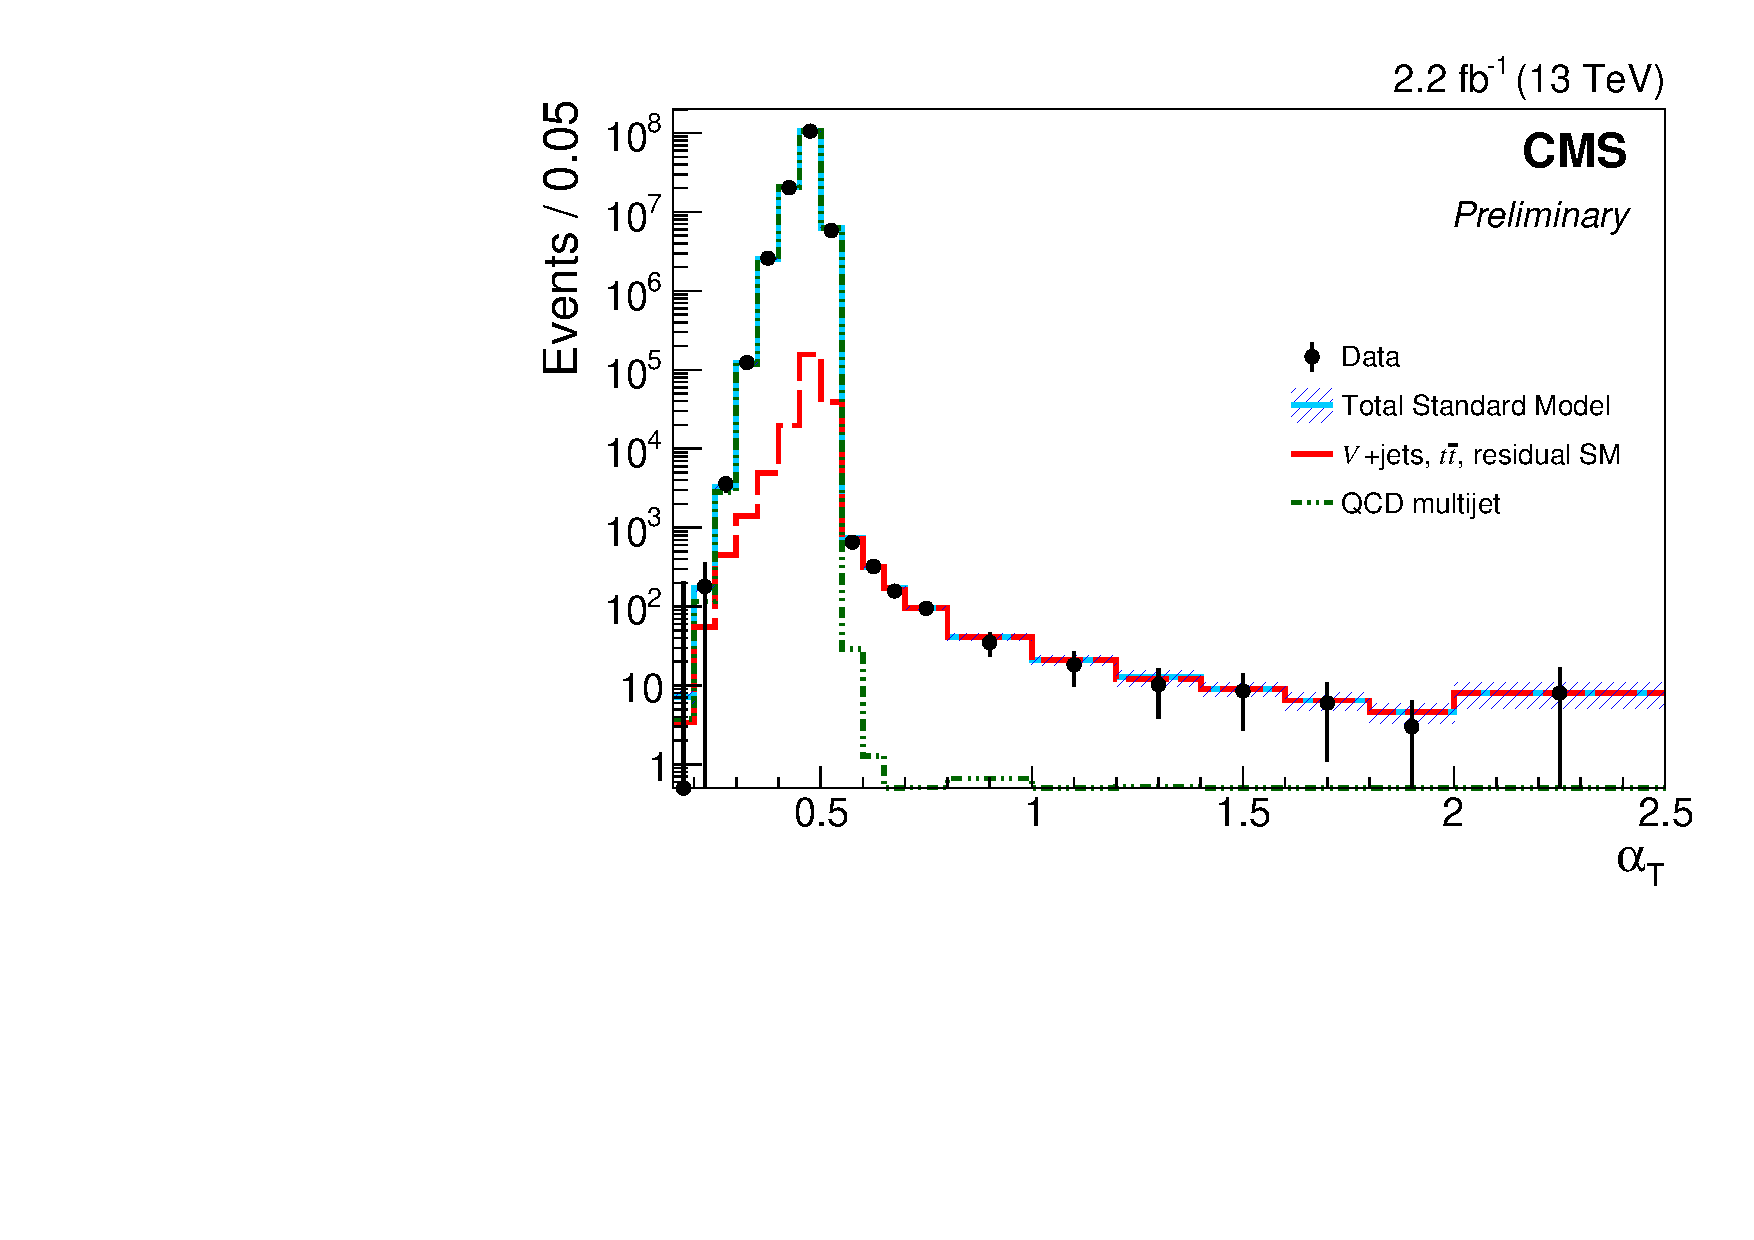
\includegraphics[width=0.49\textwidth]{alphaT_v4} \,
%    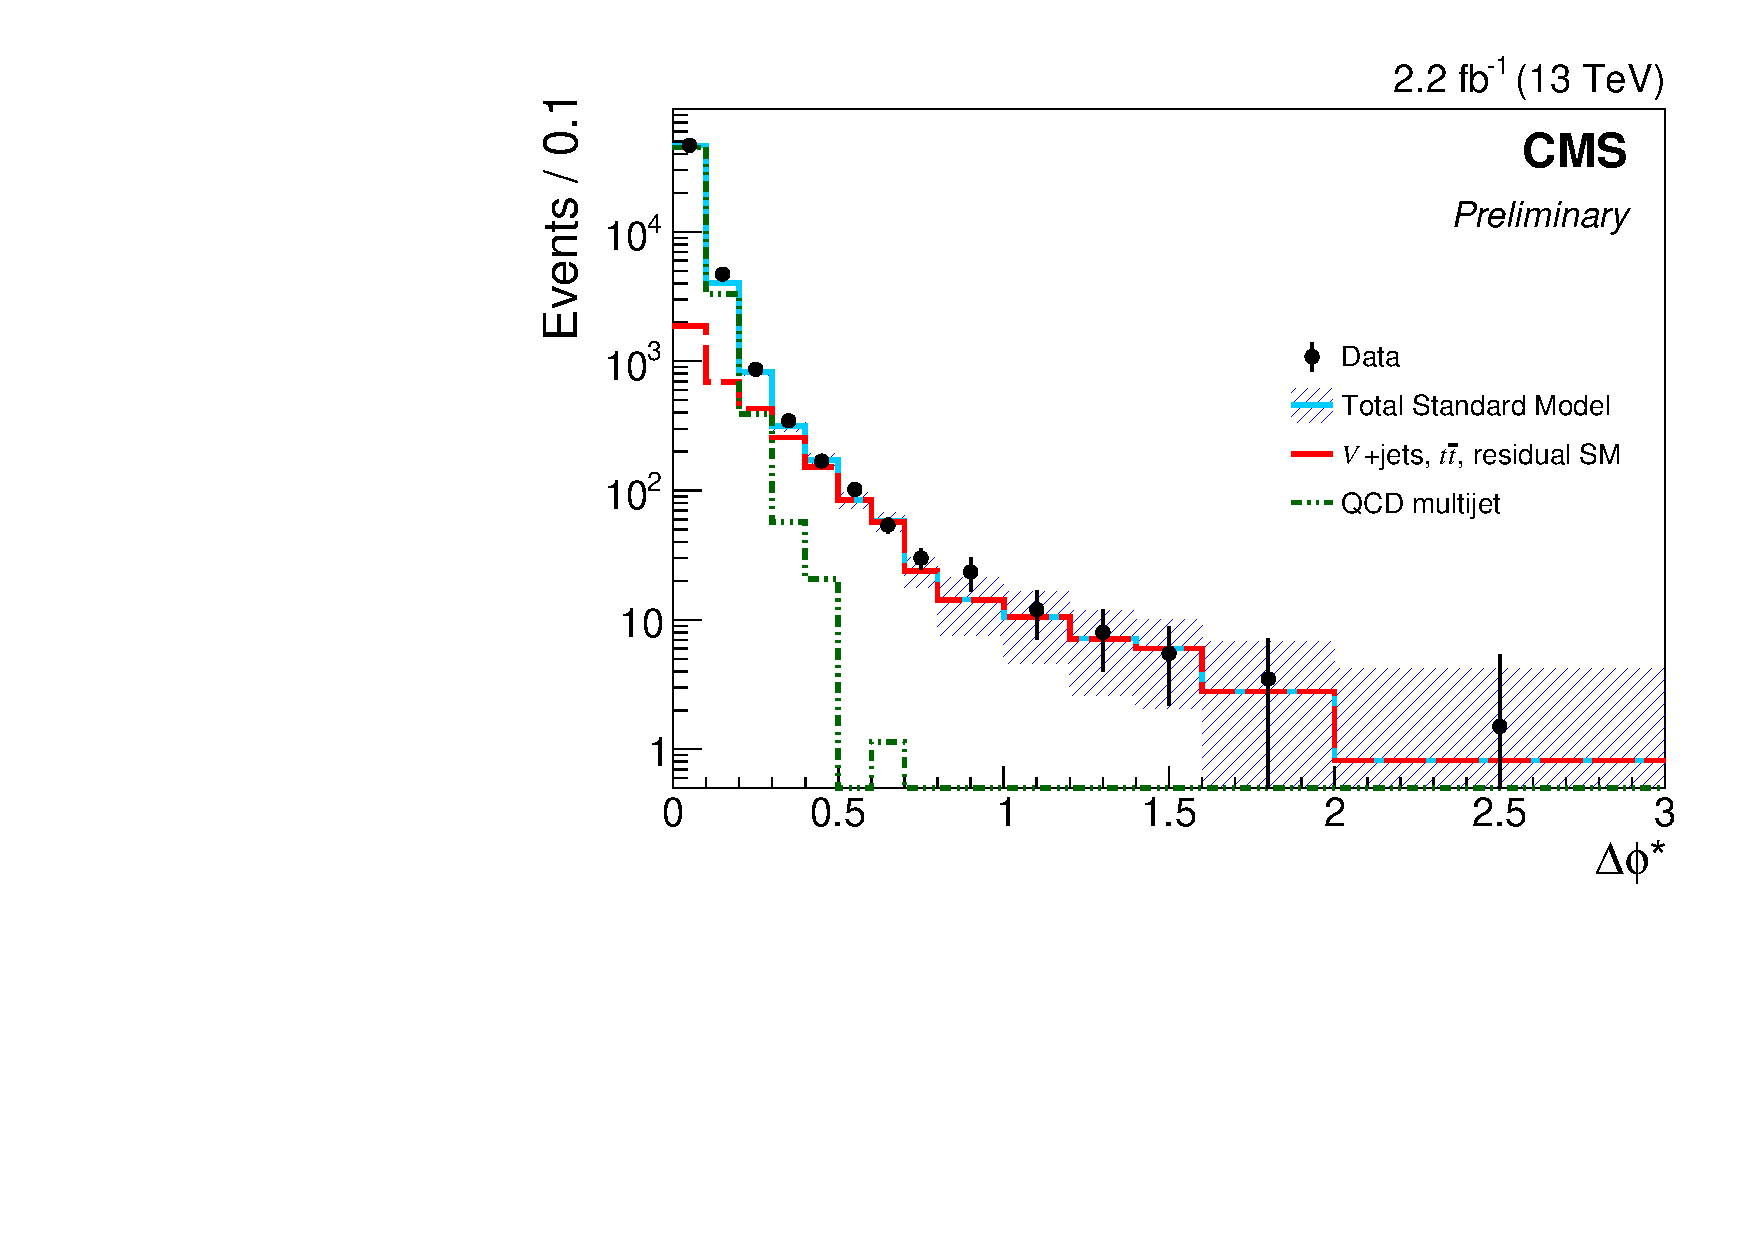
\includegraphics[width=0.49\textwidth]{bDPhi_v4} \\
%  \end{center}
%  \caption{(Left) The \alphat distribution observed in data for events
%    that are recorded with unbiased trigger conditions and satisfy the
%    baseline (full signal region) selection criteria for the region
%    $\alphat < 0.55$ ($\alphat > 0.55$). (Right) The \bdphi
%    distribution observed in data for events that satisfy the full
%    signal region selection criteria and $\scalht > 800\GeV$.  The
%    distributions for the QCD multijet backgrounds are determined from
%    simulation while all other SM backgrounds are estimated using a
%    $\mu$ + jets data control sample. %The uncertainties in the SM
%    %expectation are dominated by the statistical uncertainties 
%    %associated with the limited sample of simulated multijet events.
%    \label{fig:alphat-bdphi} 
%  }
%\end{figure*}

\begin{table}[tb!]
  \topcaption{Efficiency $\varepsilon_\textrm{trig}$ [\%] of the signal triggers as
    a function of \scalht after applying the signal region selection
    criteria, as determined from data. The first (asymmetric) and
    second set of are statistical and systematic in nature.
  } 
%  \footnotesize
  \centering
  \begin{tabular}{lcccc} 
    \hline
    \scalht [GeV]                    & 200--400 & 400--600 & 600--900 & $>$900 \\
    \hline
    $\varepsilon_\textrm{trig}$ [\%] & $97.4^{+0.5}_{-0.6}{}^{+0.6}_{-0.6}$ 
                                     & $97.9^{+0.8}_{-1.2}{}^{+1.0}_{-1.0}$ 
                                     & $100.0^{+0.0}_{-1.8}{}^{+0.0}_{-0.6}$ 
                                     & $100.0^{+0.0}_{-3.6}{}^{+0.0}_{-0.1}$ \B  \\
    \hline
  \end{tabular}
  \label{tab:triggers}
\end{table}

Candidate signal events are recorded with a number of trigger
conditions. Trigger logic requiring the presence of significant \mht
and \met is used to record events containing one or more
jets. Additional logic is used that simultaneously requires
predetermined thresholds on \scalht and \alphat to be
satisfied. Finally, a trigger condition based solely on \scalht is
used to record candidate events for the region $\scalht >
900\GeV$. The combined trigger strategy provides high efficiencies for
all event categories of the the signal region, which are primarily
dependent on \scalht, as summarised in Table~\ref{tab:triggers}.

%_______________________________________________________________________________
%_______________________________________________________________________________
%_______________________________________________________________________________

\subsection{Background composition}
\label{sec:bkgd}

Following the application of the \alphat and \bdphi variables, the
multijet background is reduced to a negligible level. The remaining
small contribution is estimated with the method described in
Sec.~\ref{sec:qcd} that relies on the multijet-enriched control sample
defined in Sec.~\ref{sec:control}.

The SM processes that provide the dominant contributions to the
background counts involve the production of high-\pt neutrinos in the
final state. The associated production of jets and Z bosons that decay
to \znunu dominate the background counts for events containing low
numbers of jets and b-tagged jets. The \znunuj background is
irreducible. 

The associated production of jets and W bosons, decaying to $\PW^\pm
\to \ell\nu$ ($\ell=\Pe$, $\Pgm$, $\Pgt$), is also a significant
background in the same phase space. The production and semileptonic
decay of top quark-antiquark pairs (\ttbar) to W bosons and b quarks
becomes the dominant background process for events containing high
numbers of jets or b-tagged jets. Residual contributions from other
processes, such as single top production, WW, WZ, ZZ (diboson)
production, and the associated production of \ttbar and a boson
({\ttbar}W, {\ttbar}Z, {\ttbar}$\gamma$, and {\ttbar}H), may also lead
to W bosons in the final state. Events that contain the leptonic decay
of a W boson are typically rejected by the vetoes that identify the
presence of leptons or single isolated tracks. If the lepton is
outside the experimental acceptance, or is not reconstructed or
isolated, then the event is not vetoed and the aforementioned
processes lead to what is collectively known as the ``lost lepton''
(\lost) background.

The \lost and \znunuj backgrounds are estimated with the methods
described in Sec.~\ref{sec:ewk} using control samples of \mj and \mmj
events, respectively, as defined in Sec.~\ref{sec:control}.

%_______________________________________________________________________________
%_______________________________________________________________________________
%_______________________________________________________________________________

\subsection{Control regions}
\label{sec:control}

Three control regions are used to estimate the SM backgrounds in the
signal region. Kinematic requirements ensure the control samples are
enriched in the same or similar SM processes that populate the signal
region, and are depleted in contributions from SUSY models (\ie
so-called signal contamination). The event selection requirements for
the three control samples are summarised in
Table~\ref{tab:selections}.

The first control region comprises a multijet-enriched sample of
multijet events. The selection criteria are identical to the signal
region requirements except for the $\mhtmet$ and $\bdphi$
requirements, which are inverted. The control region is defined by
sidebands that satisfy $1.25 < \mhtmet < 3.0$ and $0.2 < \bdphi <
0.5$. The events are recorded with the signal triggers described
above.

Two additional control samples comprising \mj or \mmj events are
defined by the application of the baseline selection criteria and
requirements on isolated, central, high-\Pt muons. The selection
criteria are chosen to ensure the kinematic properties of events in
the \mj and \mmj control regions and signal region are comparable once
the muon or dimuon system is ignored in the calculation of event-level
quantities such as \scalht and \mht.

The \mj event sample is enriched in \wmj and \ttbar production, with
contributions from other rare processes such as single top and diboson
production. The sample is defined by the common preselection
requirements, but the muon veto is inverted and each event is required
to contain a single isolated muon, as defined in
Section~\ref{sec:reconstruction}, that satisfies $\pt > 30\gev$ and
$\abs{\eta} < 2.1$ and is well separated from each jet $\mathrm{j}_i$
in the event according to $\Delta R(\mu,\mathrm{j}_i) > 0.5$. The
transverse mass formed by the muon \pt and \ptvecmiss system must
satisfy $30 < m_\mathrm{T} < 125\GeV$ to select a sample of events
rich in W bosons, produced promptly or from the decay of top quarks.

The \mmj sample is enriched in the production of dimuon final states
from Z boson decays ($\PZ\! \rightarrow\!  \mu^+\mu^-$). Events from
the \znunuj and \zmumuj processes have similar kinematic properties
when the muons are ignored. The sample uses a similar set of selection
criteria as the \mj sample, but specifically requires two oppositely
charged isolated muons that both satisfy $\pt > 30\gev$ and
$\abs{\eta} < 2.1$ and are well separated from the jets in the event
($\Delta R(\mu_{1,2},\mathrm{j}_i) > 0.5$). The muons are also
required to have a dilepton invariant mass within a $\pm 25\GeV$
window around the mass of the Z boson~\cite{1674-1137-38-9-090001}.

For both the muon and dimuon samples, no requirement is made on
\alphat nor \bdphi in order to increase the statistical precision of
the predictions from these samples. Both the \mj and \mmj samples are
recorded using a trigger that requires an isolated muon. The selection
criteria of the \mj and \mmj event samples are chosen so that the
trigger is maximally efficient, with values of $\sim$90\% and
$\sim$99\%, respectively.

%_______________________________________________________________________________
%_______________________________________________________________________________
%_______________________________________________________________________________

\subsection{Categorisation of candidate signal events}
\label{sec:categorisation}

Candidate signal events, as well as events in the control regions, are
categorised according to \njet, the number of jets identified
(``tagged'') as originated from b quarks \nb, \scalht, and \mht. The
categorical binning scheme is determined primarily by the statistical
power of the \mj and \mmj event samples.

Seven bins in \njet are considered, as summarised in
Table~\ref{tab:selections}. Events that contain only one jet ($\njet =
1$) satisfying the requirement $\Pt > 40\GeV$ are labelled as
``monojet''. Events containing two or more jets are categorised
according to the \Pt of the second-most energetic jet. Events that
satisfy $\njet \geq 2$ with only the most energetic jet satisfying
$\Pt > 100\GeV$ are labelled as ``asymmetric''. Events for which the
second-most energetic jet also satisfies $\Pt > 100\GeV$ are labelled
as ``symmetric'' and are categorised according to \njet (2, 3, 4, 5,
and $\geq$6). The symmetric topology targets the pair production of
SUSY particles and their cascade decays, while the monojet and
asymmetric topologies target nearly mass-degenerate SUSY models, as
well as the direct production of weakly interacting massive particles.

\begin{table}[!tb]
  \topcaption{Lower bound for the final open \scalht bin [GeV] used in
    the search as a function of \njet and \nb. A dash (--) signifies a
    category that is not used. The label {\it a} signifies the
    asymmetric topology. 
}
  \label{tab:categorisation}
  \centering
  \begin{tabular}{ lccccc }
    \hline
    $\njet\, / \,\nb$ & 0         & 1         & 2         & 3         & $\geq$4 \\
    \hline
    1                 & \ph{1}900 & \ph{1}900 & --        & --        & --      \\ 
    $\geq$2{\it a}    & \ph{1}900 & \ph{1}900 & \ph{1}900 & \ph{1}600 & --      \\ 
    2                 & 1200      & 1200      & \ph{1}900 & --        & --      \\ 
    3                 & 1200      & 1200      & 1200      & \ph{1}900 & --      \\ 
    4                 & 1200      & 1200      & 1200      & \ph{1}900 & --      \\ 
    5                 & 1200      & 1200      & 1200      & \ph{1}900 & 400     \\ 
    $\geq$6           & 1200      & 1200      & 1200      & 1200      & 400     \\ 
    \hline
  \end{tabular}
\end{table}

%\begin{table}[!tb]
%  \topcaption{Lower bound for the final open \scalht bin [GeV] used in
%    the search as a function of \njet and \nb. A dash (--) signifies a
%    category that is not used. The label {\it a} signifies the
%    asymmetric topology. 
%}
%  \label{tab:categorisation}
%  \centering
%  \begin{tabular}{ lccc }
%    \hline
%    $\njet\, / \,\nb$ & 0         & 1         & $\geq$2   \\
%    \hline
%    1                 & \ph{1}900 & \ph{1}600 & --        \\ 
%    $\geq$2{\it a}    & \ph{1}900 & \ph{1}900 & \ph{1}400 \\ 
%    2                 & 1200      & 1200      & \ph{1}200 \\ % CHANGE TO 400!
%    3                 & 1200      & 1200      & \ph{1}600 \\ 
%    4                 & 1200      & 1200      & \ph{1}900 \\ 
%    5                 & 1200      & 1200      & \ph{1}900 \\ 
%    $\geq$6           & 1200      & 1200      & \ph{1}900 \\ 
%    \hline
%  \end{tabular}
%\end{table}

Events are also categorised according to \nb (0, 1, 2, 3, $\geq$4),
where \nb is bounded from above by \njet. The nomimal binning scheme
for \scalht is defined as follows: four bounded bins that satisfy
200--400, 400--600, 600--900, and 900--1200\GeV, and a final open bin
$\scalht > 1200\GeV$, which is adapted per (\njet, \nb) category as
follows. Only the region $\scalht > 400\GeV$ is considered for events
that satisfy $\njet \geq 4$. Bins at high \scalht are merged with
lower-\scalht bins to satisfy a threshold on the minimum number of
events in all bins of the control regions. These adjustments ensure
well populated control regions that are used to estimate the SM
backgrounds and validate assumptions in the likelihood model. The
boundaries of the final open \scalht bins as a function of \njet and
\nb are summarised in Table~\ref{tab:categorisation}.

Finally, the \mht variable is also used to categorise events as
follows: three bounded bins that satisfy 200--400, 400--600, and
600--900, and a final open bin $\scalht > 900\GeV$. 
%The \mht binning depends on \njet and \scalht, while an identical
%binning scheme is used across all \nb categories. 
The \mht binning depends on \njet, \scalht, and \nb. 
The maximum value for \mht is bounded from above for \scalht bins that
are also bounded. High \mht bins are merged such that the lower bound
of the final bin is limited to that of the \scalht bin, if below
900\GeV. The \mht variable is not employed for monojet events, for
which \mht is equivalent to \scalht, or events that satisfy $200 <
\scalht < 400\GeV$.

\begin{table}[!tb]
  \topcaption{Variables used to categorise events for the signal and
    control regions and the total number of bins. 
%    The number in parentheses represent the maximum number of bins
%    possible for each variable.   
  }
  \label{tab:catfinal}
  \centering
  \begin{tabular}{ llc }
    \hline
    Region    & Variables                                 & Bins     \\
    \hline
    Signal    & \njet, \scalht, \nb, \mht                 & 274      \\
    \mj       & \njet, \scalht, \nb                       & 207      \\
    \mmj      & \njet, \scalht                            & \ph{2}61 \\
    Multijet  & \njet, \scalht                            & \ph{2}30 \\
%    Signal   & \njet (7), \scalht (5), \nb (5), \mht (4) & 274      \\
%    \mj      & \njet (7), \scalht (11), \nb (5)          & 207      \\
%    \mmj     & \njet (7), \scalht (11)                   & \ph{2}61 \\
%    Multijet & \njet (7), \scalht (5)                    & \ph{2}30 \\
    \hline
  \end{tabular}
\end{table}

Based on this categorisation scheme, there are 274 bins in the signal
region. The categorisation of the control event samples is discussed
below. The number of bins for all samples is summarised in
Table~\ref{tab:catfinal}. 

%_______________________________________________________________________________
%_______________________________________________________________________________
%_______________________________________________________________________________

\subsection{Categorisation of control event samples}
\label{sec:categorisationcr}

The control regions employ similar event categorisation schemes to
that used for the signal region, as described in the following. Events
in the signal and the three control regions are identically
categorised according to \njet.

The multijet control region uses an \scalht binning identical to the
signal region, while the \mj and \mmj control regions use a more
granular binning scheme. Up to eleven bins are used to determine the
SM background estimates, which are then aggregated to match the five
\scalht bins used for the signal region.  This approach allows to
correct simulated event samples based on granular measurements
determined from the data control regions, which in turn improves the
modelling of the SM backgrounds. The \scalht binning scheme is shown
in Table~\ref{tab:thresholds}. 

Events in the signal and \mj control region are also identically
categorised according to \nb, while the multijet event sample is
categorised inclusively with respect to \nb, and the \mmj events are
subdivided according to the following scheme: $\nb = 0$ and $\nb \geq
1$. Hence, templates determined from simulation are used in
conjunction with the transfer factors from the multijet and \mmj
control regions to predict the background counts in the \mht
dimension for the regions $\nb \geq 0$ and $\nb \geq 1$, respectively.  

Finally, event counts in the three control regions are integrated over
\mht. Hence, simulation-based templates are also utilised in
conjunction with the transfer factors from all control regions to
predict the background counts in the \mht dimension.

%_______________________________________________________________________________
%_______________________________________________________________________________
%_______________________________________________________________________________

%\subsection{Simplified binning scheme}
%\label{sec:aggregated}
%
%Data counts and SM background estimates are aslo provided for an
%alternate, simplified binning scheme in which events are organised
%into eight distinct topologies defined in terms of \njet and \nb, as
%summarised in Table~\ref{tab:aggrsr}. For each topology, event yields
%are integrated over the full \scalht range, $\scalht > 200\GeV$, and
%categorised according to the four bins in \mht defined above. This
%scheme leads to 32 bins that are exclusive, contiguous, and provide a
%complete coverage of the signal region. The SM background estimates
%are based on the same likelihood model used to determine the nominal
%result.
%
%\begin{table}[!tb]
%  \centering
%  \caption{The event topologies, defined in terms of
%    requirements on \njet and \nb, for the simplified binning
%    scheme. Events are further categorised according to four \mht bins
%    per topology.
%    \label{tab:aggrsr}
%  }
%  \begin{tabular}{lccc}
%    \hline
%    Topology     & \njet categories  & Low \nb & High \nb \\
%    \hline
%    Monojet-like & 1, $\geq$2{\it a} & 0--1    & $\geq$2  \\
%    Low \njet    & 2, 3              & 0       & $\geq$1  \\
%    Medium \njet & 3, 4              & 0--1    & $\geq$2  \\
%    High \njet   & 5, $\geq$6        & 0--2    & $\geq$3  \\
%    \hline
%  \end{tabular}
%\end{table}

%_______________________________________________________________________________
%_______________________________________________________________________________
%_______________________________________________________________________________

%\clearpage
\section{Monte Carlo simulation}
\label{sec:simulation}

The search relies on several event samples, recorded by the CMS
experiment or simulated with Monte Carlo (MC) generator programs, to
estimate the backgrounds from various SM processes.

The {\MADGRAPH{}5\_a\MCATNLO} 2.2.2~\cite{Alwall2014} event generator
is used at leading order (LO) accuracy to produce samples of \wj, \zj,
\ttbar, and multijet events. The same generator is used at
next-to-leading order (NLO) accuracy to generate samples of s-channel
production of single top, as well as {\ttbar}W, {\ttbar}Z, and
{\ttbar}$\gamma$ events. The NLO \POWHEG v2~\cite{powheg,
  powheg_top_Wt} generator is used to describe the t- and tW-channel
production of events containing single top quarks, as well as
{\ttbar}H events. The \PYTHIA 8.2~\cite{pythia} program is used to
generate diboson (WW, WZ, ZZ) production. The simulated samples are
normalised according to production cross sections that are calculated
with NLO and next-to-NLO precision~\cite{Alwall2014, wphys, fewz,
  wwxs, top++, nlotop, powheg_top_Wt}. Simulated \wj and \zj events
are weighted according to the true vector boson \Pt obtained from the
{\MADGRAPH{}5\_a\MCATNLO} generator code (used at LO) to account for
the effect of missing NLO QCD and electroweak (EWK) terms in the
matrix element calculation. Events from the \ttbar simulated samples
are weighted to improve the description of jets arising from initial
state radiation. The description of the detector response, for these
SM processes, is implemented using the \GEANTfour~\cite{geant}
package.

Event samples for signal models involving the gluino-mediated or
direct pair production of squarks, in association with up to two
additional partons, are generated at leading order with
{\MADGRAPH{}5\_a\MCATNLO}, and the decay of the sparticles is
performed with \PYTHIA 8.2~\cite{pythia}. Inclusive,
process-dependent, signal production cross sections are calculated
with NLO plus next-to-leading-logarithm (NLL)
accuracy~\cite{Beenakker:1996ch, PhysRevLett.102.111802,
  PhysRevD.80.095004, 1126-6708-2009-12-041,
  doi:10.1142/S0217751X11053560, susynlo}. The detector response is
provided by the CMS fast simulation package~\cite{fastsim}.

The \textsc{NNPDF}3.0 LO and \textsc{NNPDF}3.0 NLO~\cite{nnpdf} parton
distribution functions (PDF) are used, respectively, with the LO and
NLO generators described above. The \PYTHIA 8.2~\cite{pythia} program
is used to describe parton showering and hadronisation for all
simulated samples. To model the effects of multiple pp collisions
within the same or neighboring bunch crossings (pileup), all simulated
events are generated with a nominal distribution of pp interactions
per bunch crossing and then reweighted to match the pileup
distribution as measured in data.

%_______________________________________________________________________________
%_______________________________________________________________________________
%_______________________________________________________________________________

\section{Non-multijet background evaluation}
\label{sec:ewk}

The \lost and \znunuj backgrounds are estimated using data control
regions and ``transfer factors'' determined from simulation: 

\begin{align}
  \tf^{\lost} \, & = \,
  \frac{\mathcal{N}^{\lost}_\textrm{MC}(\njet, \scalht, \nb, \mht)}
  {\mathcal{N}^{\mj}_\textrm{MC}(\njet, \scalht, \nb)\hfill} \; ;
  & 
  \mathcal{N}^{\lost}_\textrm{pred} \, & = \,
  \tf^{\lost} \; \mathcal{N}^{\mj}_\textrm{data} \; ,
  \\
  \tf^{\znunu} \, & = \,
  \frac{\mathcal{N}^{\znunu}_\textrm{MC}(\njet, \scalht, \nb, \mht)}
  {\mathcal{N}^{\mmj}_\textrm{MC}(\njet, \scalht, \nb)\hfill} \; ;
  & 
  \mathcal{N}^\textrm{\znunu}_\textrm{pred} \, & = \,
  \tf^{\znunu} \; \mathcal{N}^{\mmj}_\textrm{data} \; ,
\end{align}

where $\tf^{\lost}$ and $\tf^{\znunu}$ are the transfer factors that
act as multiplier terms on the event counts
$\mathcal{N}^{\mj}_\textrm{data}$ and
$\mathcal{N}^{\mmj}_\textrm{data}$ observed in each (\njet, \scalht,
\nb) bin of, respectively, the \mj and \mmj control regions to
estimate the \lost or \znunuj background counts
$\mathcal{N}^{\lost}_\textrm{pred}$ and
$\mathcal{N}^{\znunu}_\textrm{pred}$ in the corresponding (\njet,
\scalht, \nb, \mht) bins of the signal region. The categorisation of
the \mj and \mmj event samples is described in
Sec.~\ref{sec:categorisationcr}.

\begin{table}[t!]
  \caption{
    Systematic uncertainties in the background evaluation. The quoted
    ranges are representative of the minimum and maximum variations
    observed across all bins of the signal region. The two ranges
    quoted for uncertainties derived from closure tests in data
    correpond to variations as a function of \njet and \scalht.
  } 
  \label{tab:bkgd_systs}
  \centering
  \footnotesize
  \begin{tabular}{ lcc }
    \hline
    Source of uncertainty\T\B           & Magnitude (\%)                                  \\
    \hline
    Finite-size simulated samples\T     & 1--100                 & 1--100                 \\
    \multicolumn{3}{l}{\bf Uncertainties in corrections applied to simulation:}\T\B       \\
    Minimum bias cross section (pileup) & 0.6--3.8               & 2.3--2.8               \\
    $\mu_R$ / $\mu_F$ scales            & 2.3--3.6               & X--Y                   \\
    Parton density functions            & 1.1--2.7               & X--Y                   \\
    \wj cross section                   & 0.2--1.4               & --                     \\
    \ttbar cross section                & 0.0--1.0               & --                     \\
    QCD + EWK NLO corrections           & 0.5--5.4               & 2.2--14.3              \\
    ISR (\ttbar)                        & 0.8--1.1               & --                     \\
    Signal trigger efficiency           & 0.0--3.1               & 0.0--2.0               \\
    Muon trigger and selection          & 0.0--2.1               & 0.0--4.2               \\
    Lepton vetoes                       & X--Y                   & X--Y                   \\
    Jet energy scale                    & 3.4--5.5               & 5.3--8.0               \\
    b quark tag efficiency              & 0.4--0.6               & 0.3--0.6               \\
    b quark mistag probability          & 0.1--1.4               & 0.2--1.8               \\
    \multicolumn{3}{l}{\bf Uncertainties determined from closure tests in data:}\T\B      \\
    \alphat extrapolation               & 3--\ph{2}9, 2--\ph{1}6 & 3--\ph{2}9, 2--\ph{1}6 \\
    \bdphi extrapolation                & 2--22, 1--18           & 2--22, 1--18           \\
    W boson polarisation                & 1--\ph{2}7, 1--\ph{1}7 & --                     \\
    Single isolated track veto          & 0--10, 0--13           & --                     \\
    \multicolumn{3}{l}{\bf Validation of \mht modelling against control data:}\T\B        \\
    \mht modelling\B                    & 0--30                  & 0--50                  \\
    \hline
  \end{tabular}
\end{table}

Several sources of uncertainty in the transfer factors are evaluated.
In addition to statistical uncertainties arising from finite-size
simulated event samples, the most relevant systematic effects are
discussed below, and generally fall into one of three categories. The
first category concerns uncertainties in ``scale factor'' corrections
applied to simulation, which are determined using inclusive data
samples that are defined by loose selection criteria, to account for
the mismodelling of theoretical and experimental parameters. The
second category concerns ``closure tests'' in data that probe specific
extrapolations or assumptions made in the analysis. Finally, the third
category concerns the use of multiple data control samples are used to
evaluate the degree to which the simulation describes the \mht
distributions observed in data, and to assign appropriate systematic
uncertainties in addition to known theoretical and experimental
uncertainties.

%    QCD + EWK NLO corrections           & 0.5--5.4           & 2.2--14.3             \\
%    $N_\textrm{isr}$ (\ttbar)           & 0.8--1.1           & --                    \\
%    Signal trigger efficiency           & 0.0--3.1           & 0.0--2.0              \\
%    Muon trigger and selection          & 0.0--2.1           & 0.0--4.2              \\
%    Lepton vetoes                       & X--Y               & X--Y                  \\
%    Jet energy scale                    & 3.4--5.5           & 5.3--8.0              \\
%    b-quark tag efficiency              & 0.4--0.6           & 0.3--0.6              \\
%    b-quark mistag probability          & 0.1--1.4           & 0.2--1.8              \\

The uncertainties from known theoretical and experimental sources are
propagated through to the transfer factors and \mht and \nb templates
to ascertain the magnitude of variations related to: the jet energy
scale, the efficiency and misidentification probability of b quark
jets, the efficiency to trigger on and identify, or veto,
well-reconstructed, isolated leptons, the inclusive W boson and \ttbar
production cross sections~\cite{}, the parton density
functions~\cite{}, the renormalisation and factorisation scales, and
the modelling of initial state radiation in addition to \ttbar
production~\cite{}. Uncertainties in the NLO and EWK NLO corrections
to the \wj and \zj simulated samples, as well as ISR with \ttbar
production, are also considered. A 5\% uncertainty in the minimum bias
cross section~\cite{} is assumed and propagated through to the
reweighting procedure to account for differences between the simulated
and data-derived measurements of the pileup
distributions. Uncertainties in the signal trigger efficiency
measurements are also propagated to the transfer factors. The effect
of the aforementioned systematic uncertainties are summarised in
Table~\ref{tab:bkgd_systs}, in terms of representative ranges.  Each
source of uncertainty is assumed to vary with a fully correlated
behaviour across the full phase space of the signal and control
regions.

Sources of additional uncertainties are determined from ``closure
tests'' that aim to identify \njet- or \scalht-dependent sources of
systematic bias arising from extrapolations performed by transfer
factors. Each closure test uses the observed event counts in up to
eleven bins in \scalht, integrated over \njet and \nb, in the \mj and
\mmj control samples to obtain a prediction of the observed yields in
another control sample. The extrapolation is performed by transfer
factors. Any nonclosure between the data count and prediction per
\scalht bin is assigned as a systematic uncertainty, uncorrelated
between \scalht bins and fully correlated between \njet and \nb
categories. The same closure tests are also performed based on event
counts in each of the seven \njet event categories, integrated over
\scalht and \nb, to determine \njet-dependent systematic uncertainties
fully correlated between \scalht bins and \nb categories. Several sets
of tests are performed. The accuracy of the modelling of the
efficiencies of both the \alphat and \bdphi requirements are estimated
from both the \mj and \mmj samples. The effects of W polarisation are
probed by using \mj events with a positively charged muon to predict
those containing a negatively charged muon. Finally, the efficiency of
the single isolated track veto is also probed using a sample of \mj
events. The uncertainties are summarised in
Table~\ref{tab:bkgd_systs}.

Finally, the \mht templates from simulation are compared to the
distributions observed in the control samples, and inspected for
trends, by assuming a linear behaviour of the ratio of observed and
simulated counts as a function of \mht. Linear fits are performed
independently for each \njet category while integrated event counts
over \nb and \scalht, and the repeated for each \scalht bin while
integrated event counts over \njet and \nb, in a procedure analogous
to that performed for the closure tests. Systematic uncertainties are
determined from any nonclosure between data and simulation. The
uncertainties, which can be as large as $\sim$50\% in the most
sensitive \mht bins, are summarised in Table~\ref{tab:bkgd_systs}.

%_______________________________________________________________________________
%_______________________________________________________________________________
%_______________________________________________________________________________

\section{Multijet background evaluation}
\label{sec:qcd}

The multijet background is estimated by using three multijet-enriched
sidebands to the signal region defined in terms of the variables
\mhtmet and \bdphi. The sidebands are defined as follows. The
``\mhtmet'' sideband comprises events that satisfy the signal region
selection criteria except for the inverted requirement $1.25 < \mhtmet
< 5.0$. The ``\bdphi'' sideband is defined similarly, except for the
inverted requirement $0.2 < \bdphi < 0.5$. Finally, a ``double''
sideband, for which events must satisfy the signal region selection
criteria except for both inverted requirements $1.25 < \mhtmet < 5.0$
and $0.2 < \bdphi < 0.5$.

Events in each of the three sidebands are categorised according to
\njet and \scalht. The event counts in data are corrected to account
for contamination from nonmultijet SM processes, such as vector boson
and \ttbar production, plus residual contributions from other SM
processes. The corrected counts are assumed to arise solely from
multijet production. The nonmultijet processes are estimated from the
\mj and \mmj control regions, as described in Sec.~\ref{sec:ewk}.

For each of the three sidebands, a transfer factor per (\njet,
\scalht) bin is obtained from simulation, defined as the ratio of the
number of multijet events that satisfy the sideband requirement to the
number that fail this requirement. Three estimates of the multijet
background per (\njet, \scalht) bin are obtained from the product of
these transfer factors and the corrected data counts from the three
sidebands. The multijet background is found to be small, typically at
the percent level, relative to the sum of all other SM backgrounds in
all (\njet, \nb) bins of the signal region.

Statistical uncertainties as large as $\sim$100\%, associated with the
finite event counts in data and simulated event samples, are
propagated to each estimate. Uncertainties as large as $\sim$20\% in
the estimates of nonmultijet contamination, determined following the
prescriptions described in Sec.~\ref{sec:ewk}, are also propagated to
the corrected events. Finally, differences between the three estimates
per (\njet, \scalht) bin are adequately covered by a systematic
uncertainty of 100\% assumed to be uncorrelated for different (\njet,
\scalht) bins.

Finally, the distribution of multijet events as a function of \nb and
\mht per (\njet, \scalht) bin is assumed to be identical to the
distribution expected for the nonmultijet backgrounds. This final
assumption is based on studies in simulation and is a valid
simplification given the magnitude of the multijet background relative
to the sum of all other SM backgrounds, as well as the magnitude of
the statistical and systematic uncertainties in the estimates
described above.

%_______________________________________________________________________________
%_______________________________________________________________________________
%_______________________________________________________________________________

\section{Results}
\label{sec:result}

A likelihood model of the observations in all data samples is used to
obtain a consistent prediction of the SM backgrounds and to test for
the presence of a variety of signal models.  In each bin of \scalht
for events in the same category of \njet and \nb, the observation is
modelled as a Poisson-distributed variable around the sum of the SM
expectation (and a potential signal contribution). The SM expectation
is related to the expected yields in the \mj and \mmj control samples
via the transfer factors derived from simulation. Likelihood functions
describe the yields in the \scalht bins of the \mj and \mmj control
samples in the same category of \njet and \nb as the signal
region. The systematic uncertainties summarised in
Table~\ref{tab:bkgd_systs} are accommodated in the likelihood function
by nuisance parameters, the measurements of which are assumed to
follow a gaussian distribution.

The expected number of events from SM processes is determined from a
simultaneous fit to data in the two control regions (``CR-only fit''),
as well as a fit including the signal region (``full fit''). The
likelihood function is maximised over all fit parameters under the
SM-only hypothesis. Figures~\ref{fig:mono}--\ref{fig:sym} summarise,
respectively, the observed number of candidate signal events and the
SM expectations from the CR-only fit, in the monojet, asymmetric, and
symmetric topologies. No significant tension is observed between the
predictions and data in the signal region, which is well described by
the SM-only hypothesis.

\begin{figure}[!tb]
  \begin{center}
    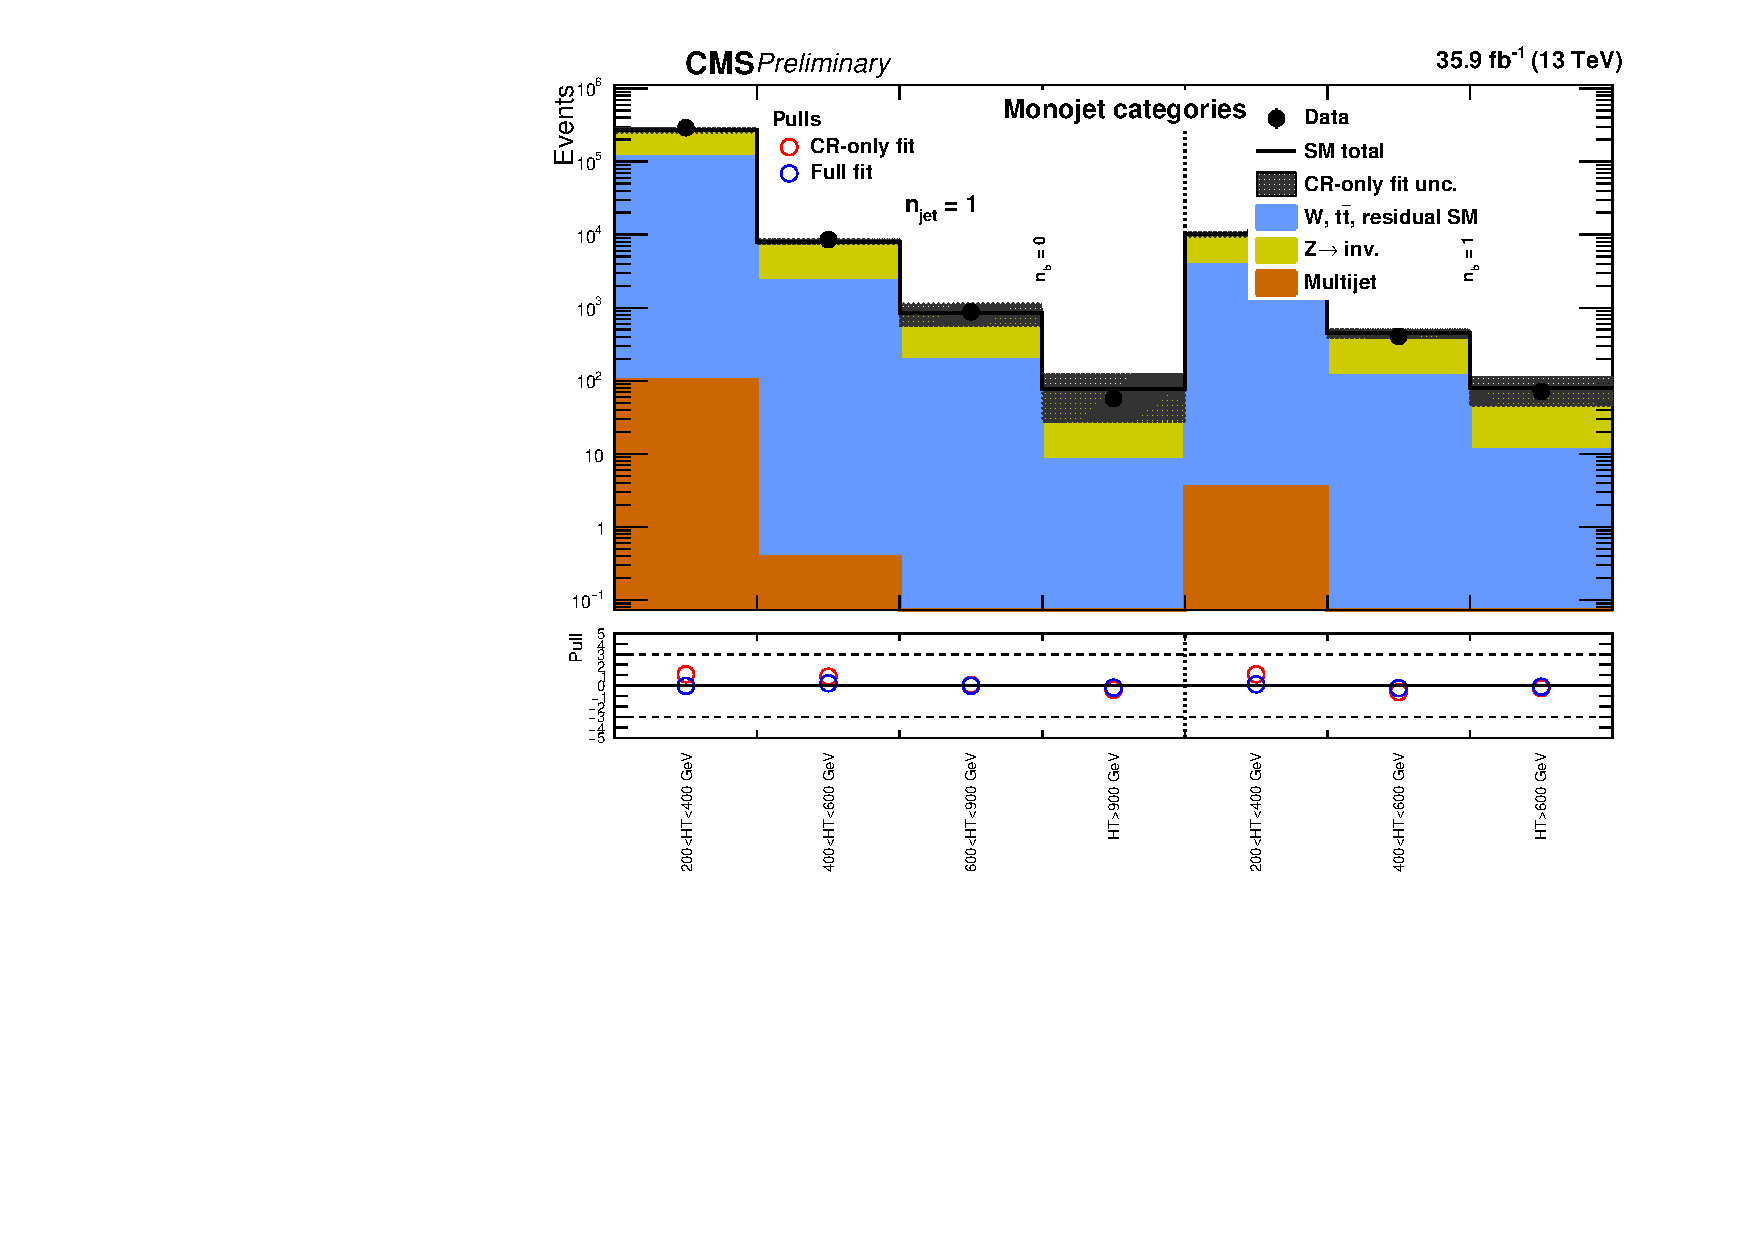
\includegraphics[width=0.7\textwidth]{summaryPlot_Monojet_prefit_overlay_fit_b}
    \caption{(Top panel) Event yields observed in data (solid circles)
      and SM expectations with their associated uncertainties (black
      histogram with shaded band) from a CR-only fit as a function of
      \nb and \scalht for the monojet topology ($\njet = 1$) in the
      signal region. (Bottom panel). The significance of deviations
      (pulls) observed in data with respect to the SM expectations
      from the CR-only (red circles) and full fit (blue circles). The
      pulls are indicative only and cannot be considered
      independently.}
    \label{fig:mono}
  \end{center}
\end{figure}

\begin{figure*}[!tb]
  \begin{center}
    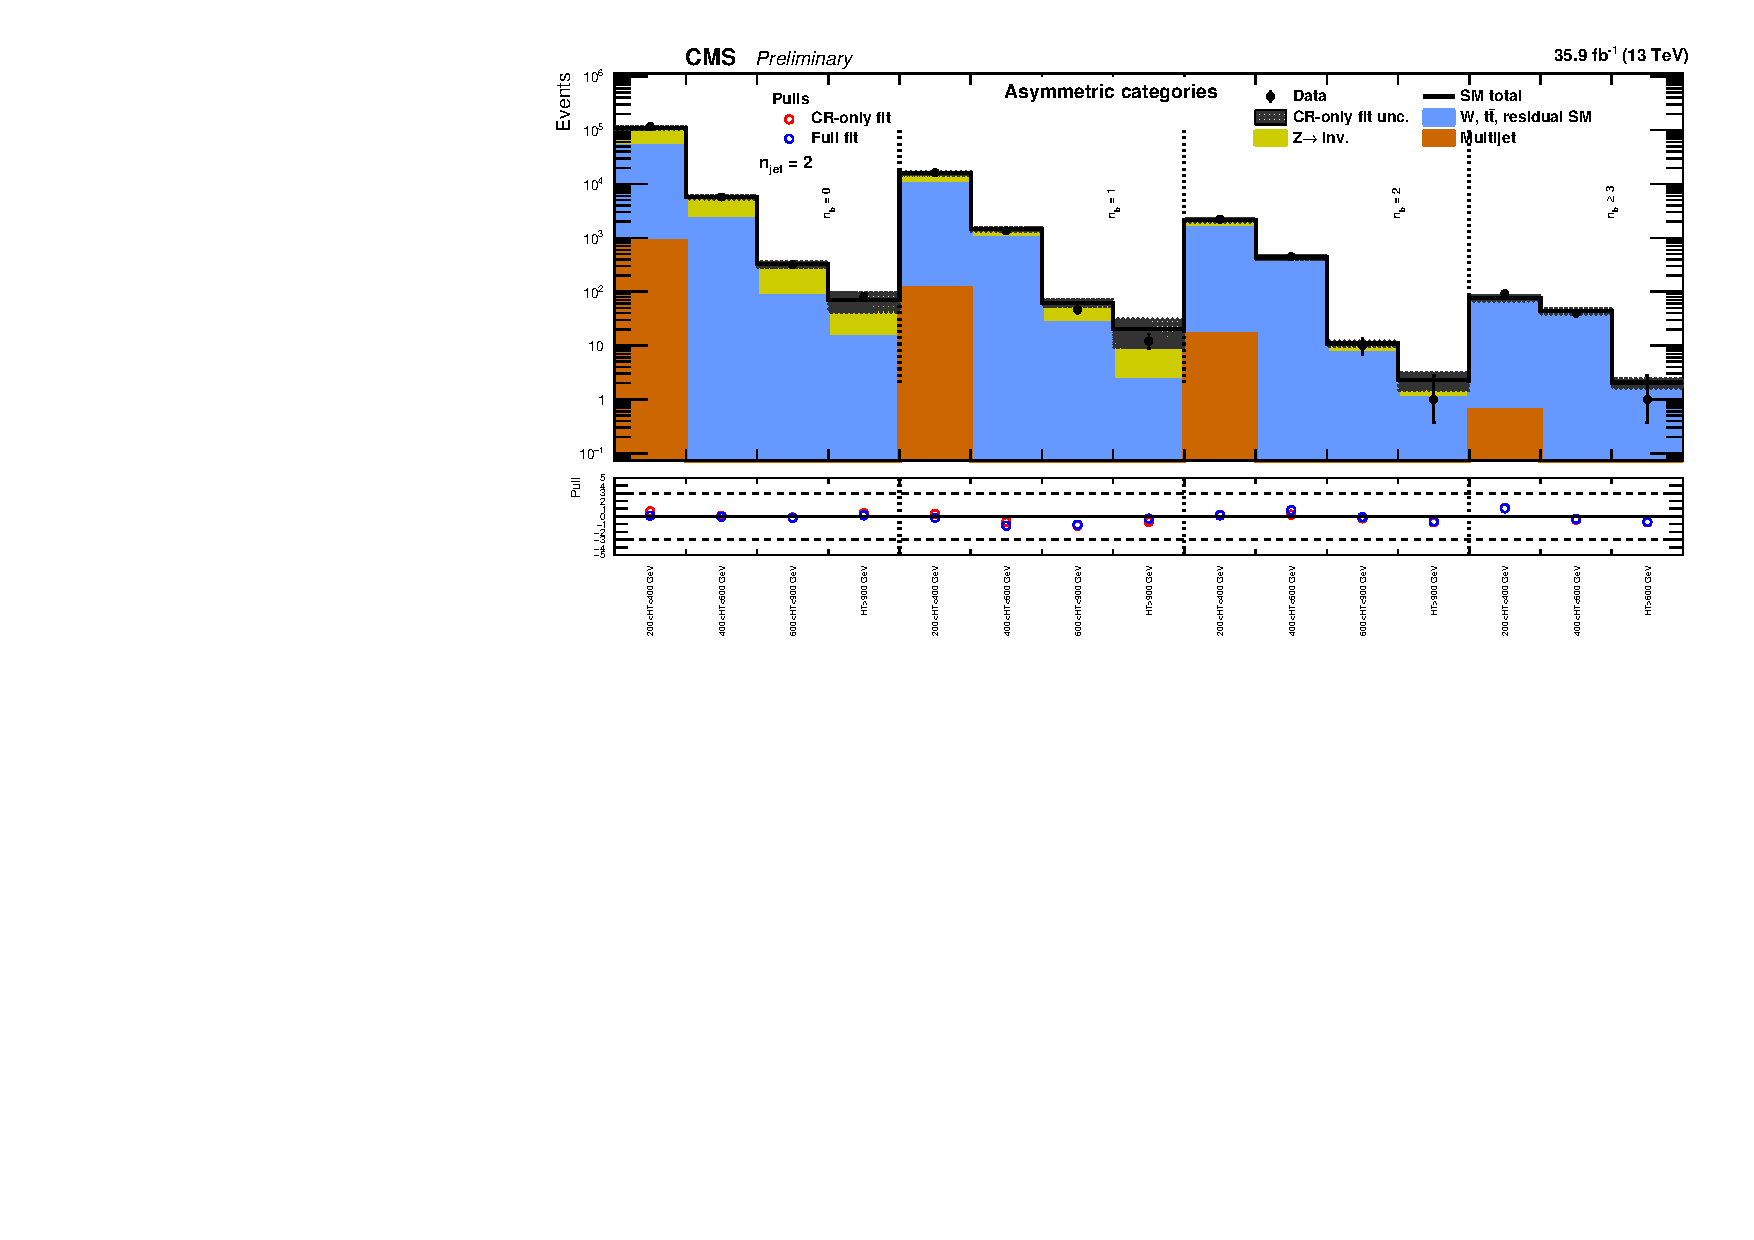
\includegraphics[width=0.7\textwidth]{summaryPlot_Asymmetric_prefit_overlay_fit_b}
    \caption{(Top panel) Event yields observed in data (solid circles)
      and SM expectations with their associated uncertainties (black
      histogram with shaded band) from a CR-only fit, integrated over
      \mht, as a function of \njet, \nb, and \scalht for the
      asymmetric topology in the signal region. (Bottom panel). The
      significance of deviations (pulls) observed in data with respect
      to the SM expectations from the CR-only (red circles) and full
      fit (blue circles). The pulls are indicative only and cannot be
      considered independently.}
    \label{fig:asym}
  \end{center}
\end{figure*}

\begin{figure*}[!tb]
  \begin{center}
    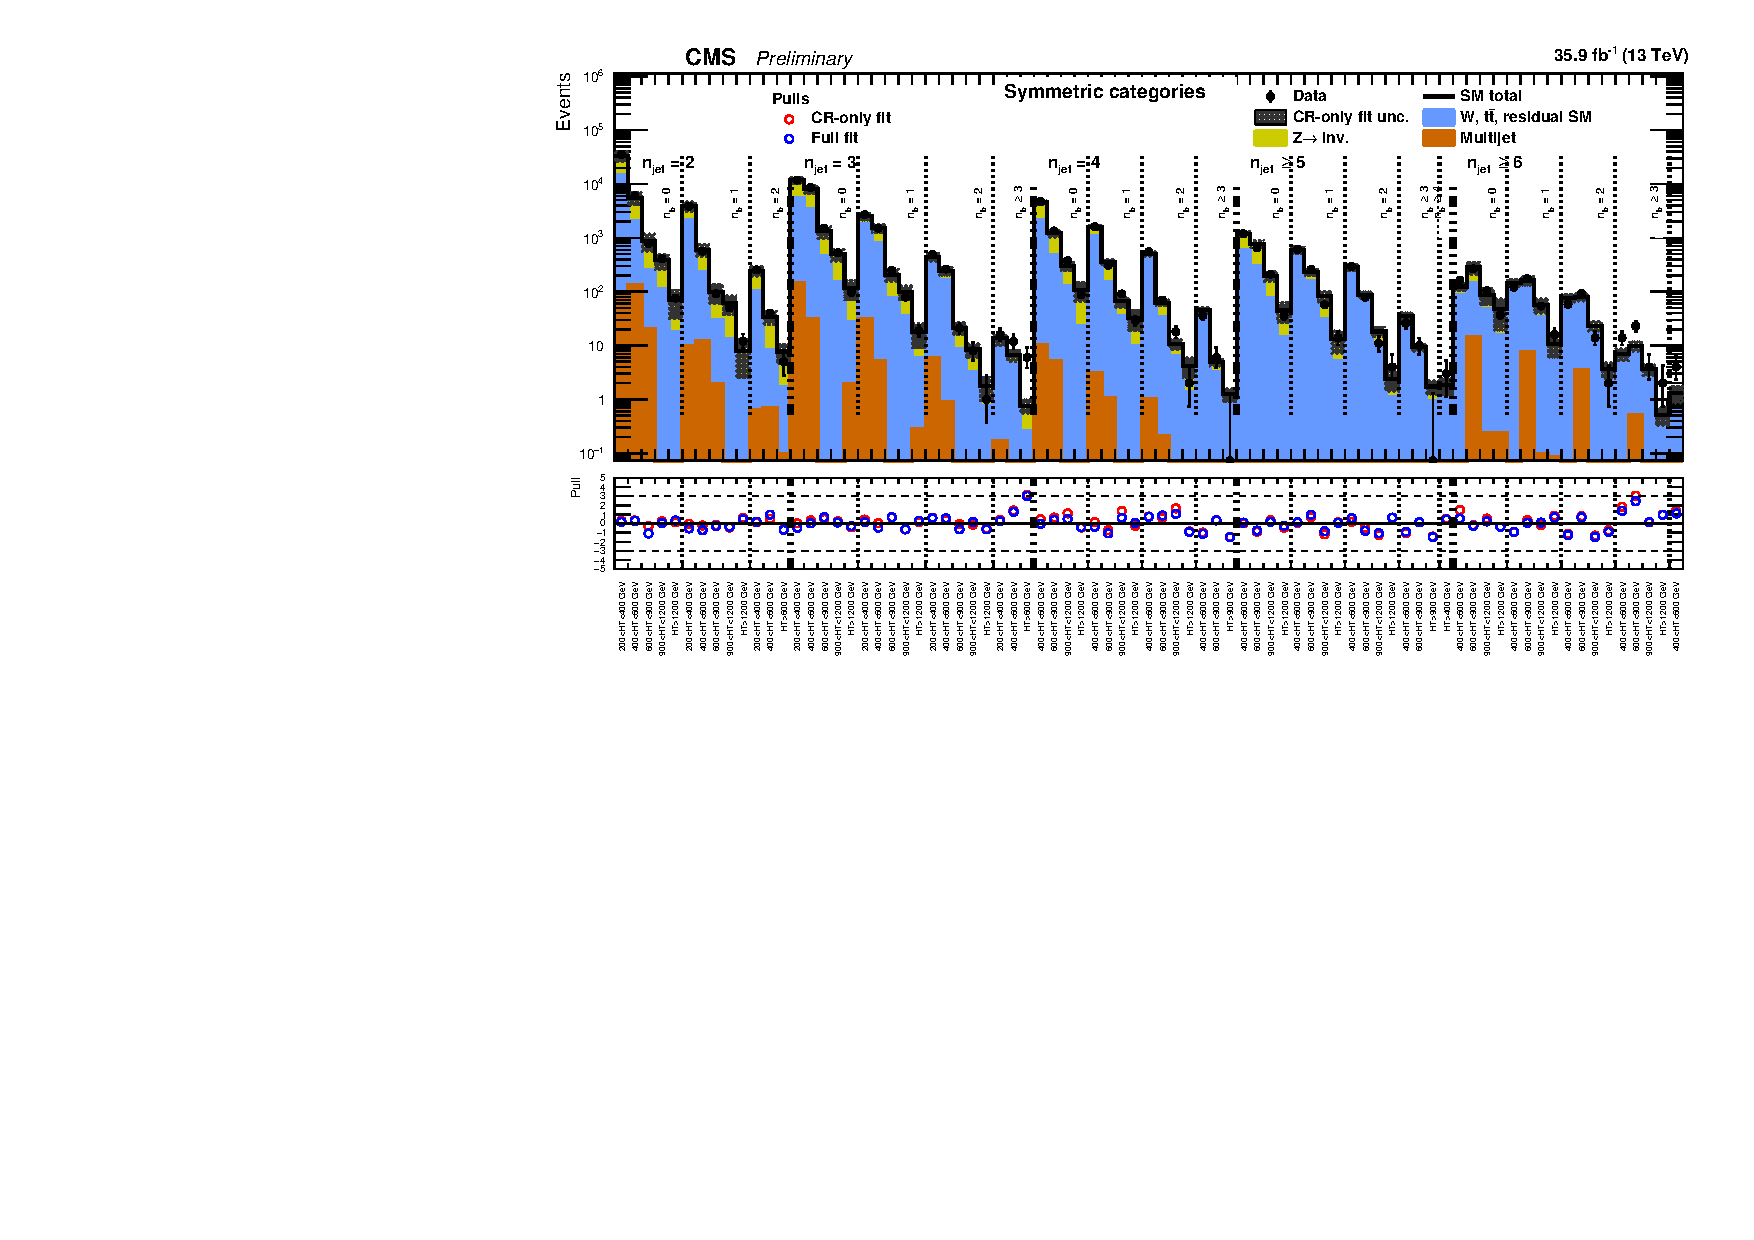
\includegraphics[angle=90,width=0.65\textwidth]{summaryPlot_Symmetric_prefit_overlay_fit_b}
    \caption{(Top panel) Event yields observed in data (solid circles)
      and SM expectations with their associated uncertainties (black
      histogram with shaded band) from a CR-only fit, integrated over
      \mht, as a function of \njet, \nb, and \scalht for the
      symmetric topology in the signal region. (Bottom panel). The
      significance of deviations (pulls) observed in data with respect
      to the SM expectations from the CR-only (red circles) and full
      fit (blue circles). The pulls are indicative only and cannot be
      considered independently.}
    \label{fig:sym}
  \end{center}
\end{figure*}

%_______________________________________________________________________________
%_______________________________________________________________________________
%_______________________________________________________________________________

\section{Interpretation}
\label{sec:interpretation}

The results of the search are used to constrain the parameter space of
simplified supersymmetric models~\cite{Alwall:2008ag, Alwall:2008va,
  sms}. Each model represents a unique production and decay mode (\ie
100\% branching ratio). The gluino-mediated or direct production of
third-generation squark pairs, and the decay of of each squark to SM
particles and the \chiz, are considered. All other sparticles are
assumed to be too heavy to be produced directly. In the case of gluino
pair production, three-body decays of the gluinos are assumed via
off-shell squarks.

Under the background + signal hypothesis, and in the presence of a
non-zero signal contribution, a modified frequentist approach is used
to determine upper limits at 95\% confidence level (CL) on the cross
section, $\sigma_\text{UL}$ (pb), to produce pairs of supersymmetric
particles as a function of the parent sparticle and the LSP
masses. The potential contributions from a new-physics signal to each
of the signal and control regions are considered, even though the only
significant contribution occurs in the signal region and not the
control region (\ie signal contamination). The approach is based on
the one-sided (LHC-style) profile likelihood ratio as the test
statistic, the \cls criterion~\cite{junk, read}, and asymptotic
formulae~\cite{Cowan:2010js} are utilised to approximate the
distributions of the test statistics under the SM background-only and
signal + background hypotheses. 

The experimental acceptance times efficiency
($\mathcal{A}\times\varepsilon$) and its uncertainty are evaluated
independently for each model as a function of the gluino or squark
mass and the \chiz mass. Several sources to the uncertainty in
$\mathcal{A}\times\varepsilon$ are considered. The effect of each
source of uncertainty on the \mht templates is evaluated from
simulated signal events, categorised according to \njet, \nb, and
\scalht. Correlations are taken into account where appropriate,
including those relevant to signal contamination that may contribute
to counts in the control samples.

\begin{table}[h!]
  \caption{
    Representative magnitudes of systematic uncertainties in the
    experimental acceptance for simplified models that assume the 
    pair production of bottom squarks and their decay to a b
    quark and a \chiz.}  
  \label{tab:signal_systs}
  \centering
  \footnotesize
  \begin{tabular}{ lccc }
    \hline
    Systematic source\T\B          & Type          & Correlated & Typical magnitude (\%) \\
    \hline
    Luminosity\T                   & Normalisation & Yes        & 2.6                    \\
    Monte Carlo statistics         & Normalisation & No         & 1--24                  \\
    Jet energy scale               & Norm. + shape & Yes        & 4--11                  \\
    b-tag efficiency scale factors & Norm. + shape & Yes        & 1--5                   \\
%    Lepton scale factors          & Normalisation & Yes        & 1--5                   \\
    Pile-up                        & Norm. + shape & Yes        & 6--10                  \\
    Trigger efficiency             & Norm. + shape & Yes        & 0--3                   \\
    Initial state radiation        & Norm. + shape & Yes        & 1--8                   \\
%    Modelling of \mht\B           & Normalisation & Yes        & 1--5                   \\
%    Renormalisation/factorisation & Norm. + shape & No         & 10                     \\
    \hline
  \end{tabular}
\end{table}

The magnitude of each contribution depends on the model and the masses
of the parent sparticle and LSP. The following sources of uncertainty
are dominant: the statistical uncertainty arising from the finite size
of simulated signal samples, the modelling of initial-state radiation
(ISR), corrections to the jet energy scale evaluated in simulation,
and the modelling of scale factors applied to simulated event samples
that correct for differences in the efficiency and misidentification
probability for b-tagged jets. The choice of PDF set, or variations
therein, predominantly affects $\mathcal{A}\times\varepsilon$ through
changes in the \Pt spectrum of the system recoil, which is covered by
the ISR uncertainty, hence no additional uncertainty is
adopted. Uncertainties in $\mathcal{A}\times\varepsilon$ due to
variations in the renormalisation and factorisation scales are
determined to be relatively small. In both cases, contributions to the
uncertainty in the theory production cross section are considered. The
uncertainty in the integrated luminosity is assumed to be
2.6\%. Representative values of the dominant systematic uncertainties
are summarised in Table~\ref{tab:signal_systs}.

\begin{figure}[!tb]
  \centering
  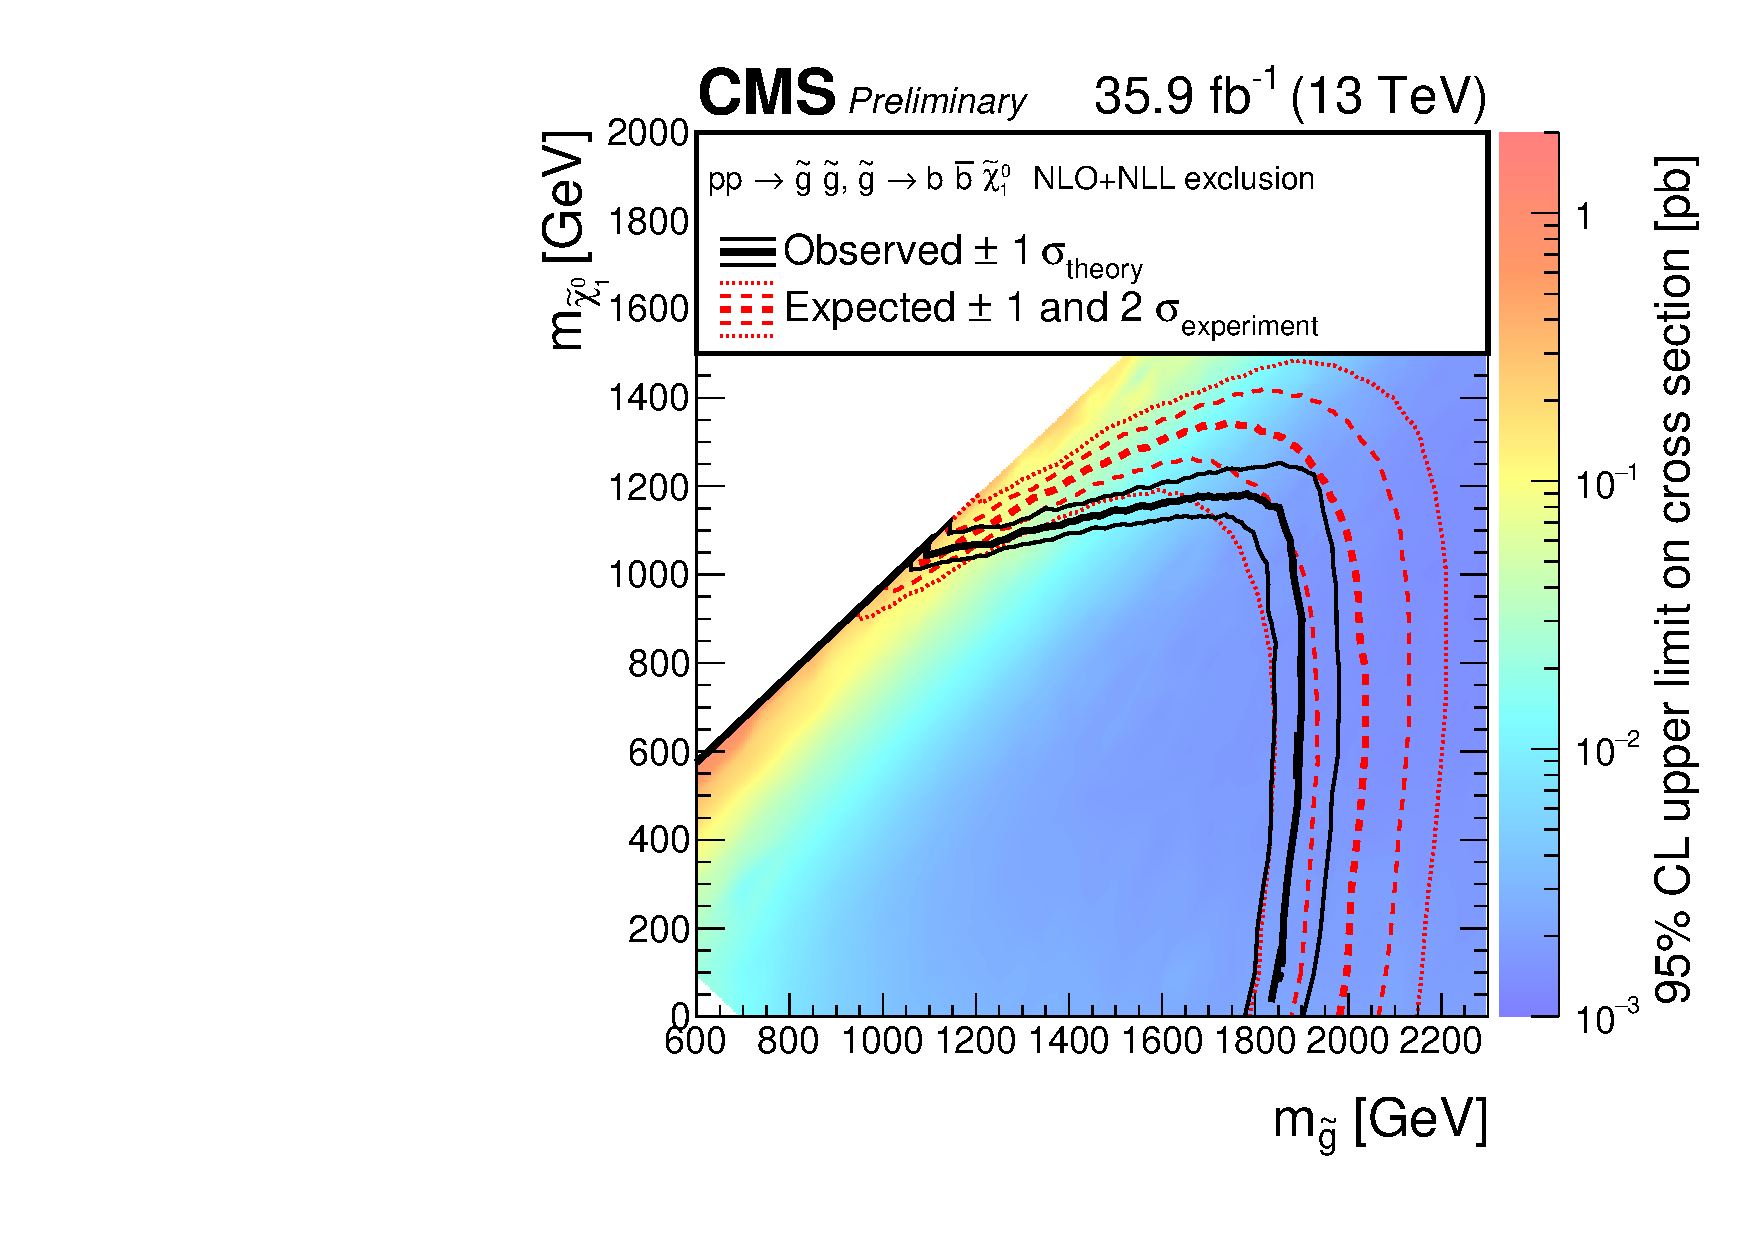
\includegraphics[width=0.49\textwidth]{T1bbbbXSEC.pdf} ~
  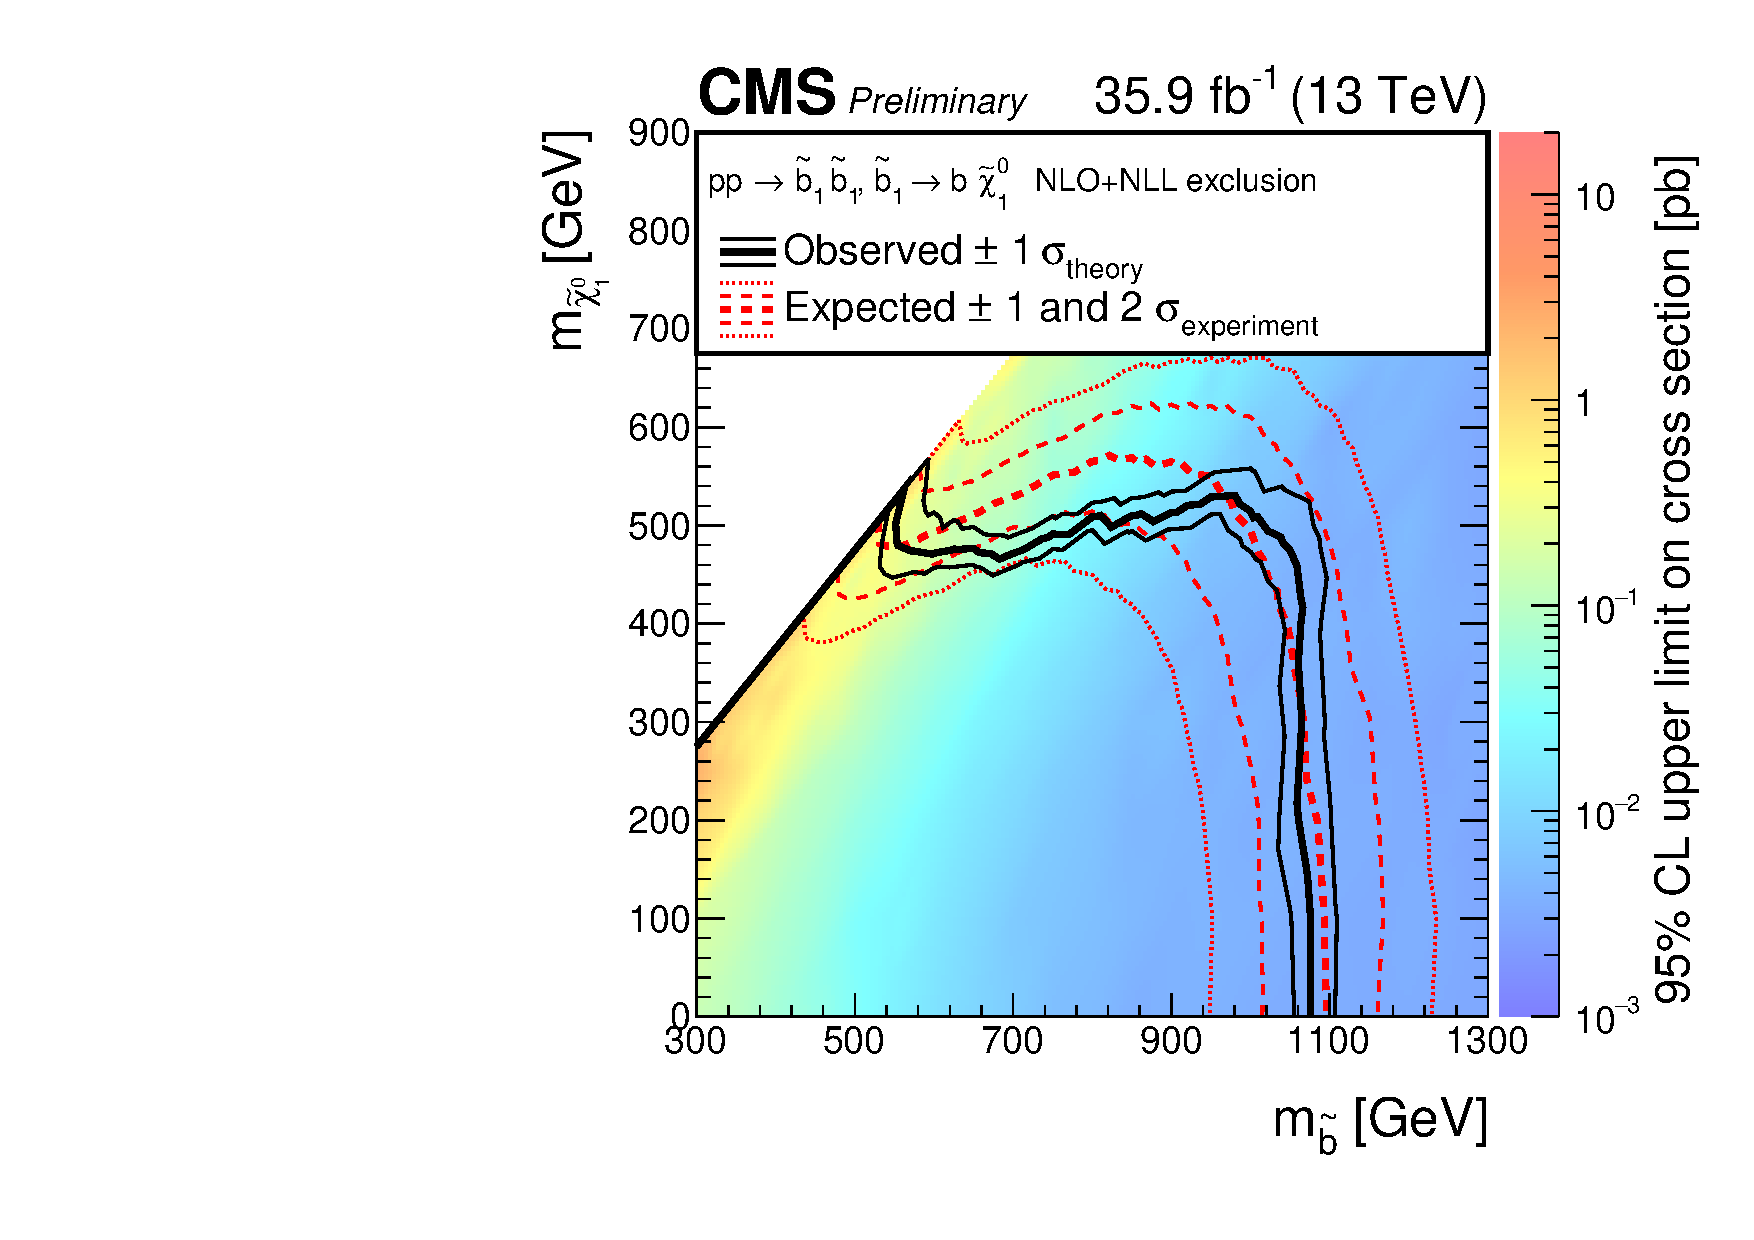
\includegraphics[width=0.49\textwidth]{T2bbXSEC.pdf} \\
  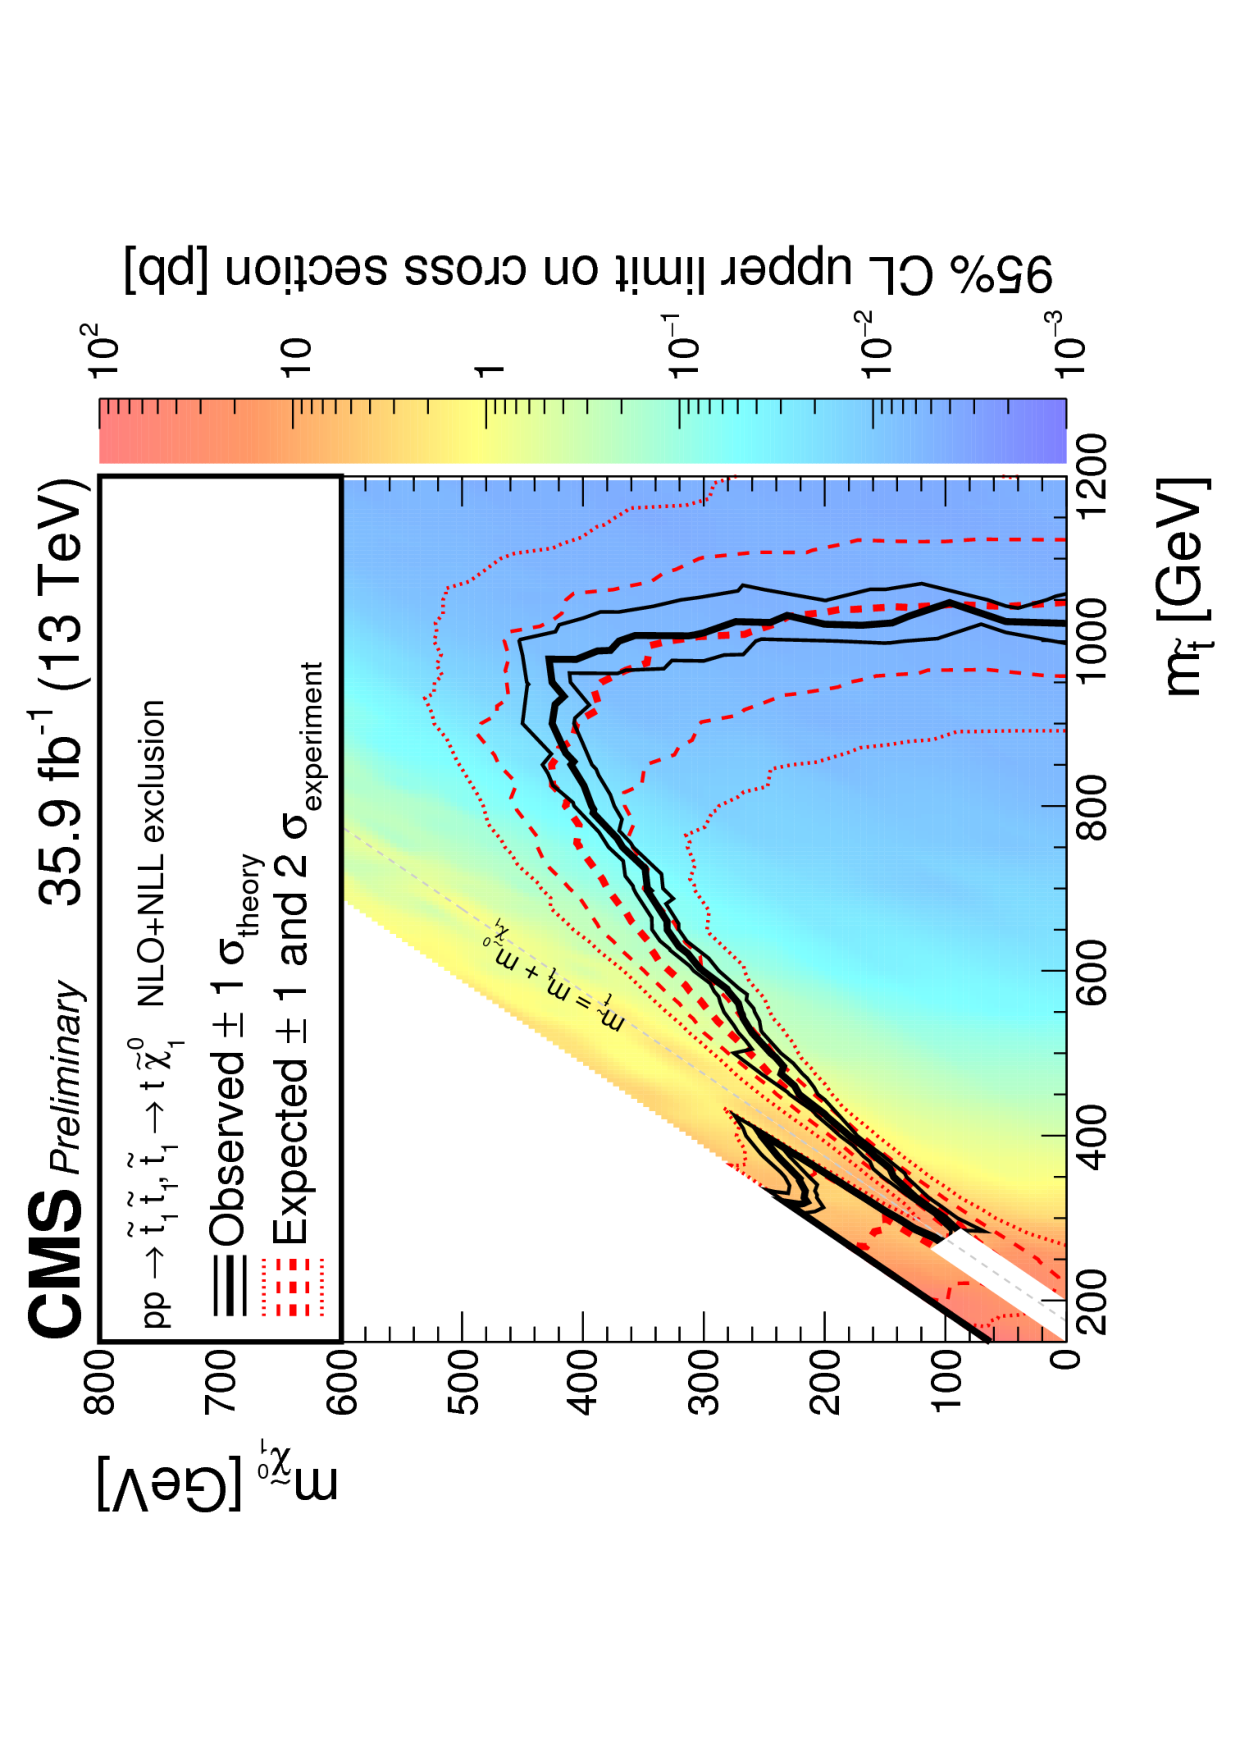
\includegraphics[width=0.49\textwidth]{T2ttXSEC.pdf} ~
  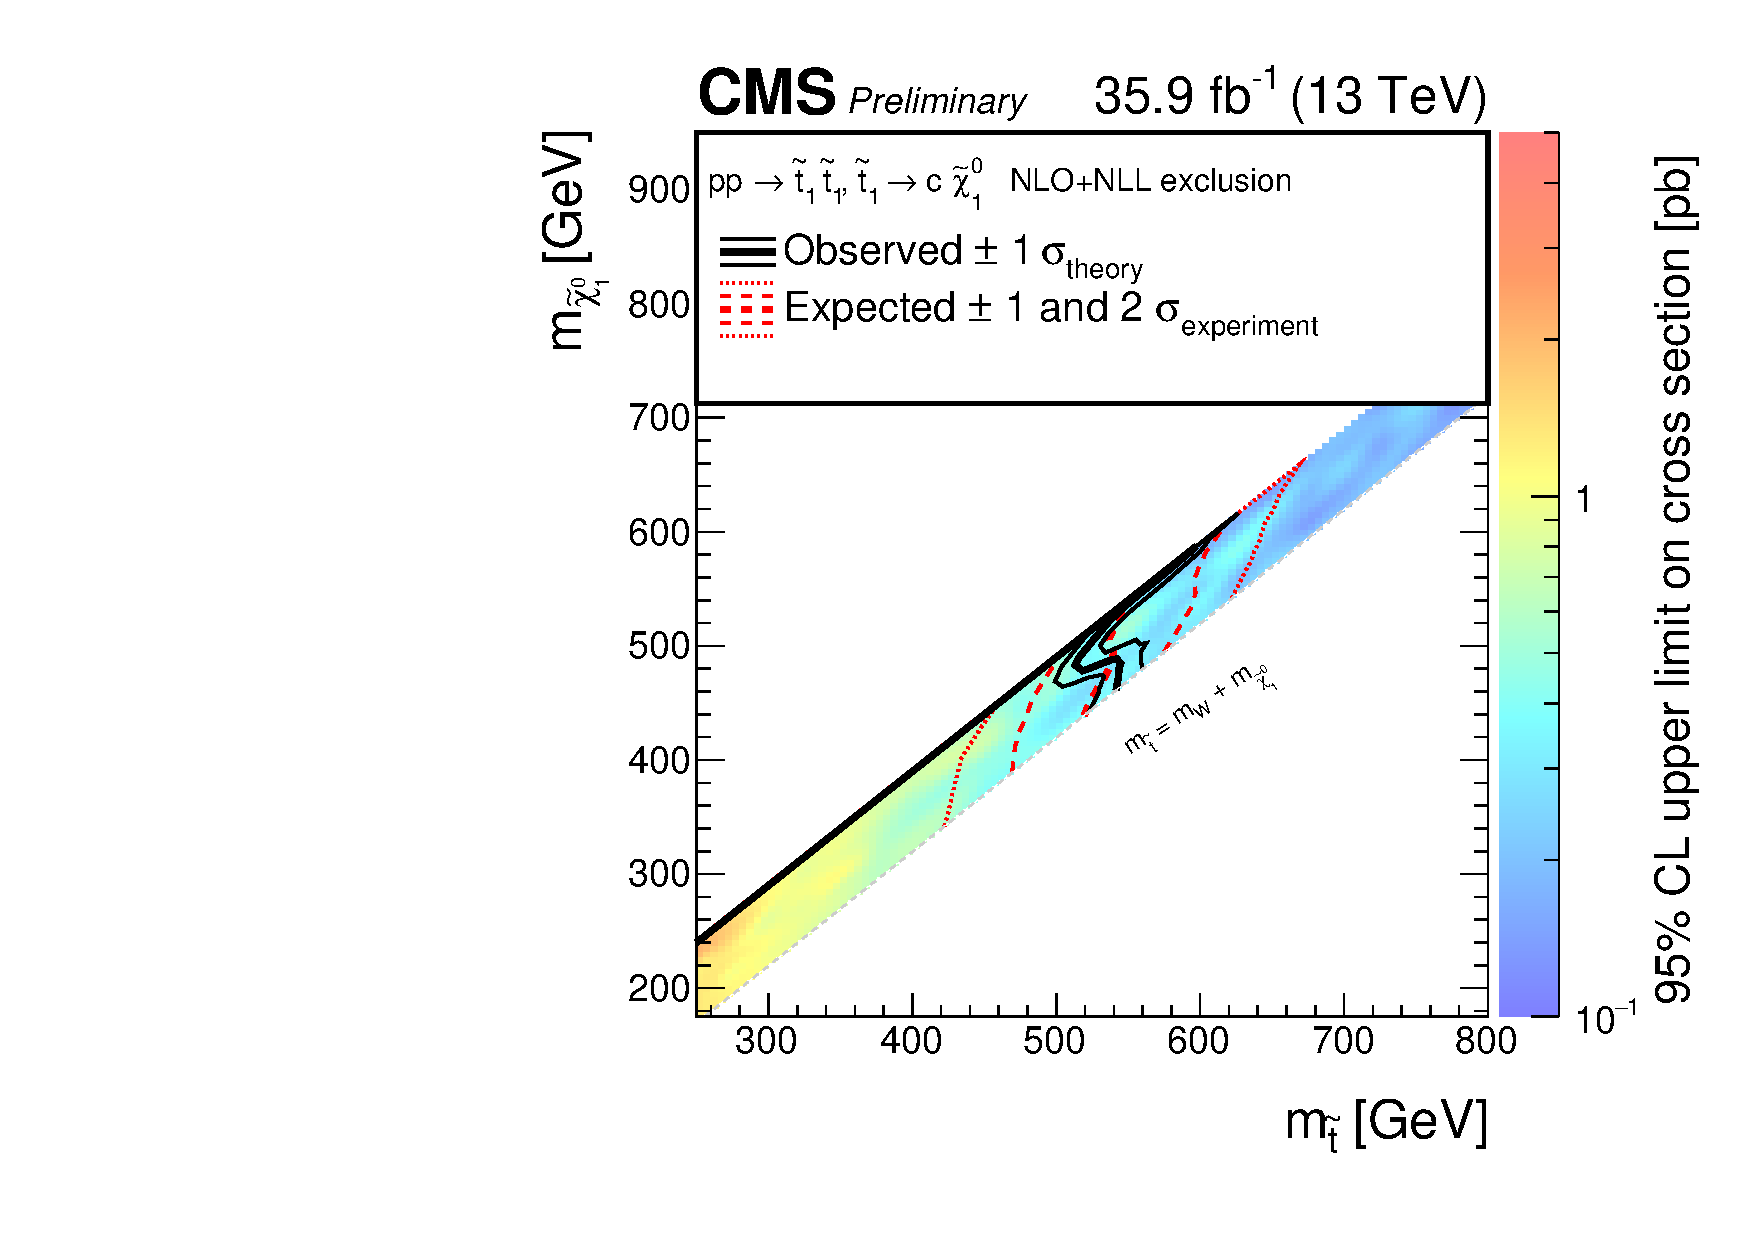
\includegraphics[width=0.49\textwidth]{T2ccXSEC.pdf} 
  \caption{Observed upper limit in cross section at 95\% confidence
    level (indicated by the colour scale) for simplified models that
    assume (Top Left) gluino-mediated and (Top Right) direct
    production of bottom squarks or the direct production of top
    squarks that each decay to (Bottom Left) the top quark or
    (Bottom Right) the charm quark and the $\chiz_{1}$, as a
    function of the gluino or squark mass and the $\chiz_{1}$ 
    mass. The black solid thick (thin) line indicates the observed
    mass exclusion regions assuming the nominal (${\pm}1 \sigma$
    theory uncertainty) production cross section. The red dashed
    thick (thin) line indicates the median (${\pm}1 \sigma$
    experimental uncertainty) expected mass exclusion
    regions. 
  }
  \label{fig:limits-sms} 
  \centering
\end{figure}

Figure~\ref{fig:limits-sms} shows the observed upper limit on the
production cross section at 95\% confidence level as a function of the
gluino or squark and \chiz masses for models that assume the
gluino-mediated or direct production of bottom and top squark
pairs. Also shown are the observed mass exclusion regions when varying
the production cross section by its theoretical uncertainty, and the
expected mass exclusion regions with the ${\pm}1$ and ${\pm}2$
standard-deviation variations.

The search places stringent limits in the mass parameter space of
these models, with observed exclusions in gluino and \chiz masses as
high as 1900 and 1175\GeV, respectively. In the case of direct
production of bottom squarks, masses as high as 1075 and 535\GeV are
excluded. Finally, top squark and \chiz masses up to 1040 and 580\GeV
are excluded. 

%A summary of the limits is provided in
%Table~\ref{tab:simplified-models-limits}.

%\newcommand{\ph}{\ensuremath{\phantom{1}}}
%\begin{table}[tb]
%  \topcaption{Summary of the mass limits obtained for the four 
%    classes of simplified models. The limits indicate the strongest
%    observed (expected) mass exclusions for the gluino or squarks, and
%    $\chiz_1$, and the quoted values have uncertainties of
%    $\pm$25\GeV.  
%  }
%  \label{tab:simplified-models-limits}
%  \centering
%  \footnotesize
%  \begin{tabular}{ llcc }
%    \hline
%    Production mode & Squark & \multicolumn{2}{c}{Strongest obs. (exp.) mass exclusion [GeV]}\T\B \\
%    \cline{3-4}                     
%                    &        & Gluino or squark\T\B & \chiz                                       \\
%    \hline                          
%    Gluino-mediated & Bottom & 1775 \ph(1850)       & 1175 \ph(1200)                              \\ 
%    Gluino-mediated & Top    & 1450 \ph(1600)       & \ph750 \ph\ph(800)                          \\ 
%    Direct          & Bottom & 1025 \ph\ph(975)     & \ph525 \ph\ph(500)                          \\ 
%    Direct\B        & Top    & \ph875 \ph\ph(925)   & \ph350 \ph\ph(350)                          \\
%    \hline
% \end{tabular}
%\end{table}

%_______________________________________________________________________________
%_______________________________________________________________________________
%_______________________________________________________________________________

\section{Summary}
\label{sec:summary}

An inclusive search for supersymmetry with the CMS experiment is
reported, based on a data sample of pp collisions collected in 2016 at
$\sqrt{s} = 13\TeV$, corresponding to an integrated luminosity of
$35.9 \pm 0.9 \fbinv$. Final states with jets and significant
\ptvecmiss, as expected from the production and decay of massive
gluinos and squarks, have been analysed. Candidate signal events are
categorised according to the number of reconstructed jets, the number
of jets identified to originate from bottom quarks, and the scalar and
vector sums of the transverse momentum of jets. The sum of standard
model backgrounds per bin has been estimated from a simultaneous
binned likelihood fit to event yields in the signal region and control
samples. The observed yields in the signal region are found to be in
agreement with the expected contributions from standard model
processes. Limits are determined in the mass parameter space of
simplified models involving the gluino-mediated and direct production
of third-generation squark pairs. The excluded mass parameter space
extends significantly beyond that set by previous searches, with
observed exclusions in gluino mass, and bottom and top squark masses,
as high as 1900, 1075, and 1040\GeV, respectively.

%_______________________________________________________________________________
%_______________________________________________________________________________
%_______________________________________________________________________________

\clearpage
\bibliography{auto_generated}








%\begin{table}[!tb]
%  \topcaption{Summary of the lower bound on \scalht [GeV] for the 
%    ({\it first, final open}) bins used in the search as a function of
%    \njet and \nb. A dash (--) signifies a category that is not
%    used. The label {\it a} signifies the asymmetric topology.
%  }
%  \label{tab:categorisation}
%  \centering
%  \begin{tabular}{ lccccc }
%    \hline
%    $\njet\, / \,\nb$ & 0                & 1                & 2                & 3                & $\geq$4    \\
%    \hline
%    1                 & (200, \ph{1}900) & (200, \ph{1}900) & --               & --               & --         \\ 
%    $\geq$2{\it a}    & (200, \ph{1}900) & (200, \ph{1}900) & (200, \ph{1}900) & (200, \ph{1}600) & --         \\ 
%    2                 & (200, 1200)      & (200, 1200)      & (200, \ph{1}900) & --               & --         \\ 
%    3                 & (200, 1200)      & (200, 1200)      & (200, 1200)      & (200, \ph{1}900) & --         \\ 
%    4                 & (400, 1200)      & (400, 1200)      & (400, 1200)      & (400, \ph{1}900) & --         \\ 
%    5                 & (400, 1200)      & (400, 1200)      & (400, 1200)      & (400, \ph{1}900) & (400, 400) \\ 
%    $\geq$6           & (400, 1200)      & (400, 1200)      & (400, 1200)      & (400, 1200)      & (400, 400) \\ 
%    \hline
%  \end{tabular}
%\end{table}

%\begin{table}[!tb]
%  \topcaption{Threshold values for the final \nb categories used in the 
%    search, as a function of \njet and the lower bounds of \scalht
%    bins [GeV]. A dash (--) signifies a (\njet, \scalht) category that
%    is not used. The label {\it a} signifies the asymmetric $\njet
%    \geq 2$ topology. The symbol $\geq$ indicates a final category
%    that covers a range of values \nb, bounded by the condition $\nb
%    \leq \njet$ unless the \njet category is also unbounded.
%  }
%  \label{tab:catttw}
%  \centering
%  \begin{tabular}{ lrrrrr }
%    \hline
%    $\njet\, / \,\scalht$ [GeV] & 200     & 400     & 600     & 900     & $>$1200 \\
%    \hline
%    1                           & 1       & 1       & 1       & $\geq$0 & --      \\ 
%    $\geq$2{\it a}              & $\geq$3 & $\geq$3 & $\geq$3 & $\geq$2 & --      \\ 
%    2                           & 2       & 2       & 2       & 2       & $\geq$1 \\ 
%    3                           & 3       & 3       & 3       & 3       & $\geq$2 \\ 
%    4                           & --      & $\geq$3 & $\geq$3 & $\geq$3 & $\geq$2 \\ 
%    5                           & --      & $\geq$4 & $\geq$3 & $\geq$3 & $\geq$2 \\ 
%    $\geq$6                     & --      & $\geq$4 & $\geq$3 & $\geq$3 & $\geq$3 \\ 
%    \hline
%  \end{tabular}
%\end{table}

%\begin{table}[!tb]
%  \topcaption{}
%  \label{tab:catzinv}
%  \centering
%  \begin{tabular}{ lrrrrr }
%    \hline
%    $\njet\, / \,\scalht$ [GeV] & 200     & 400     & 600     & 900     & $>$1200 \\
%    \hline
%    1                           & 1       & 1       & 1       & $\geq$0 & --      \\ 
%    $\geq$2{\it a}              & $\geq$2 & $\geq$2 & $\geq$1 & $\geq$1 & --      \\ 
%    2                           & 2       & $\geq$1 & $\geq$1 & $\geq$1 & $\geq$1 \\ 
%    3                           & $\geq$2 & $\geq$2 & $\geq$2 & $\geq$1 & $\geq$1 \\ 
%    4                           & --      & $\geq$2 & $\geq$2 & $\geq$2 & $\geq$1 \\ 
%    5                           & --      & $\geq$2 & $\geq$2 & $\geq$2 & $\geq$1 \\ 
%    $\geq$6                     & --      & $\geq$2 & $\geq$2 & $\geq$2 & $\geq$1 \\ 
%    \hline
%  \end{tabular}
%\end{table}
